\documentclass{article}
\PassOptionsToPackage{numbers}{natbib}
\usepackage[preprint]{neurips_2026}
\makeatletter\renewcommand{\@noticestring}{}\makeatother
\usepackage[utf8]{inputenc}
\usepackage[T1]{fontenc}
\usepackage{hyperref,xurl,booktabs,graphicx,xcolor,amsmath,array,tikz}
\usetikzlibrary{arrows.meta,positioning,shapes.geometric,calc}
\hypersetup{colorlinks=true,linkcolor=blue!45!black,citecolor=blue!45!black,urlcolor=blue!45!black,pdftitle={Lucifer-LTF: Route-Aligned Inference and Conservative Adaptation for the AlpaSim Challenge},pdfauthor={Sangram Rout}}
\newcolumntype{L}[1]{>{\raggedright\arraybackslash}p{#1}}
\newcommand{\lf}{\texttt{lf-009}}
\renewcommand{\arraystretch}{1.12}
\title{Lucifer-LTF: Route-Aligned Inference and\protect\\Conservative Adaptation for the AlpaSim Challenge}
\author{Sangram Rout\\Independent Researcher\\Team Lucifer AI (\texttt{team-lucifer})}
\date{}
\begin{document}
\maketitle
\begin{abstract}
We describe Team Lucifer AI's entries to the nuPlan track of the AlpaSim E2E Closed Loop Challenge 2026. Our final entry, \texttt{lf-013}, keeps the public py123d\_garage Latent TransFuser (LTF) checkpoint, a single-front-camera policy with a flow-matching planner, and changes only inference, in two ways. First, we correct the route interface. The simulator's route starts about 42~m ahead of the ego vehicle, and the baseline adapter took the straight-line distance to that point as distance along the road, misplacing the policy's 40/60/80~m route targets on bends. We place the targets by distance along the road and stop truncating the route at the point nearest the ego vehicle. Second, we add a bend veto. When the planned path turns by at least 10$^\circ$ and the policy's own predicted road map gives probability below 0.5 under the planned footprint, the plan is shifted sideways by 0.5 or 1.0~m, provided the shifted plan is clearly better supported and touches no predicted vehicle. Neither change reads an HD map or a logged future trajectory. On our local 1,472-scene benchmark the veto acted in 47 scenes, turned 10 off-road failures into full-score scenes and lost no full-score scene. On the post-deadline public leaderboard (November 18, 2026), \texttt{lf-013} has a mean scene score of 0.9494 and a Policy Capability Score (PCS) of 2502, the 4th-highest PCS among the best entries of the 57 participating teams. We also document what did not transfer: two earlier variants, which between them added conservative decoder-only adaptation on SimScale recovery data, plan sampling, a lead-departure rule and a 5$^\circ$ veto, raised our local mean score but received lower PCS point estimates than the route-corrected entry alone, with overlapping intervals.
\end{abstract}

% v2 planning notes (tables and figures to add) live in technical_report/TODO-v2.md, not here.
\section{Introduction}
A driving policy's small planning errors change every observation that follows, so a policy can look accurate on logged data and still fail when it drives \cite{pdm}. The AlpaSim E2E Closed Loop Challenge 2026 \cite{alpasim,board} evaluates policies in closed loop, in neural reconstructions of recorded scenes, and summarizes each entry by a Policy Capability Score (PCS), a Drive-IRT fit over all entries \cite{driveirt}, alongside the mean scene score. This report describes Team Lucifer AI's four entries to the nuPlan track, submitted between October 30 and November 17, 2026, and what their results show about which local improvements survive a hidden closed-loop benchmark.

We did not train a driving model. Every entry keeps the public py123d\_garage Latent TransFuser checkpoint \cite{garage,weights,py123d}, a roughly 68M-parameter single-camera policy, and changes how it is used: the route targets it receives, the rules applied to the poses it plans, and, for one entry, a small decoder-only adaptation on synthetic recovery data. Our local benchmark of 1,472 public scenes preferred the larger changes. The official benchmark preferred the smallest. Our contributions are:
\begin{enumerate}
\item \textbf{A route-interface correction} (\lf{}, Section~\ref{sec:route}). The served route starts about 42~m ahead of the ego vehicle. The baseline adapter took the straight-line distance to that point as distance along the road, which misplaces the checkpoint's 40/60/80~m targets on bends. We place the targets by distance along the road and keep the served route whole. On a 1,473-scene matched local panel this raised the mean score by 0.0054 and cut zero-score scenes from 62 to 52; on the October 31 official snapshot \lf{} scored 0.9454 against 0.9437 for the host's entry with the same checkpoint.
\item \textbf{A bend veto} (\texttt{lf-013}, Section~\ref{sec:veto}). When the plan bends by at least 10$^\circ$ through a region where the policy's own predicted road map gives probability below 0.5, the plan is shifted sideways by 0.5 or 1.0~m, provided the shifted plan is clearly better supported and touches no predicted vehicle. Run stand-alone on all 1,472 local scenes, the veto acted in 47, turned 10 off-road zero-score scenes into score-one scenes and lost none. Submitted as \texttt{lf-013}, it has our best official mean score (0.9494), incident distance (1.364~km) and PCS (2502), the 4th-highest PCS among the best entries of the 57 participating teams.
\item \textbf{A transfer study} (Section~\ref{sec:results}). Two entries with larger local gains, \texttt{lf-010} (decoder-only SimScale adaptation plus two inference rules) and \texttt{lf-012} (\lf{}'s weights with a lead-departure rule and a 5$^\circ$ veto), received lower PCS point estimates than \lf{} alone, and an on-policy adaptation branch inspired by RoaD produced no gain that our 48-scene comparison could resolve. We report these results in the same detail as the positive one. Appendix~\ref{app:repro} gives the submission identities and container digests of all four entries, and Appendix~\ref{app:history} the experiment history behind them.
\end{enumerate}

\section{Related work}
\paragraph{Base policy.}
TransFuser \cite{transfuser} is an imitation-learned driving policy that fuses camera and LiDAR features with transformers; its Latent TransFuser (LTF) variant is camera-only. The LTF in py123d\_garage \cite{garage,weights} adds latent bird's-eye-view features, auxiliary road-map and object heads, and a waypoint planner trained with flow matching, in the family of diffusion and flow trajectory decoders \cite{diffusiondrive,diffplanner,wamflow}. The organizers released the checkpoint we use; its card discloses pretraining on NVIDIA Physical AI AV and NuRec data \cite{nvidiadata} in addition to nuPlan \cite{nuplan,openscene}. Its auxiliary heads supply the predicted road map and object boxes that our rules read.

\paragraph{Closed-loop post-training.}
Dataset aggregation \cite{dagger} labels the states a policy reaches with an expert and retrains on them. Recent driving work applies this in reconstructed scenes: RoaD \cite{road} guides rollouts toward the logged human trajectory and fine-tunes on them, OPTED \cite{opted} labels on-policy states with a render-free teacher, and RoG-DAgger \cite{rogdagger} post-trains on guided rollouts. SimScale \cite{simscale} instead renders perturbed views of real logs and labels them with a pseudo-expert, which gives recovery data without a closed-loop rollout; LEAD \cite{lead} also trains on perturbed views of logged scenes. Our \texttt{lf-010} adaptation uses SimScale's recovery corpus, and our on-policy branch follows RoaD.

\paragraph{Rules around a learned policy.}
Other entries to this challenge pair a learned policy with a deployment-time rule. GatedVLA \cite{gatedvla} adds detector-based emergency braking to a vision-language-action policy, and Lao Siji \cite{laosiji} keeps speed control with its base model's lead-vehicle estimate behind a rule-based speed layer. Both rules act longitudinally and both entries are on the PAI-AV track. Our bend veto acts laterally, on the nuPlan track, and its trigger is the policy's own road prediction rather than a separate detector or a map.

\paragraph{Evaluation.}
Dauner et al.\ \cite{pdm} showed on nuPlan that open-loop accuracy is a weak proxy for closed-loop driving. The challenge's Drive-IRT \cite{driveirt} fits an item-response model over all entries and models zero, intermediate and score-one scene outcomes separately, so an entry's PCS depends on the whole population and is refitted as entries arrive. Section~\ref{sec:results} shows a further gap: our local mean score did not predict official PCS.

\section{Method summary}\label{sec:summary}
Figure~\ref{fig:overview} shows the deployed system. The public checkpoint runs unchanged. Our changes sit at its two interfaces: on the input side, the placement of the route targets (Section~\ref{sec:route}); on the output side, a rule layer that edits the 64 planned poses before the AlpaSim controller executes them (Sections~\ref{sec:veto} and~\ref{sec:variants}). Maps, expert futures and scene identities are absent from the deployed interface; the only perception the rules use is the policy's own output.

\begin{figure}[htbp]
\centering
% System overview figure (Figure 1), drawn in TikZ. Panel (a): lf-013 inference loop; (b) route targets on a bend;
% (c) bend veto. Panels (b) and (c) are schematic. The camera thumbnail is a frame rendered in our local AlpaSim run
% (openai_golf/lead-candidate-2026-11-07/outputs/frames/9ad434ec99685d35-CAM_F0-1017000.jpg, public track assets).
\definecolor{pubF}{HTML}{E9EFF7}\definecolor{pubB}{HTML}{8DA2C0}
\definecolor{ourF}{HTML}{FCE8DC}\definecolor{ourB}{HTML}{E0662F}
\definecolor{headF}{HTML}{F5EFDA}\definecolor{headB}{HTML}{C4B37C}
\definecolor{simF}{HTML}{F3F3F1}\definecolor{simB}{HTML}{9B9A95}
\definecolor{inkC}{HTML}{3A3A3A}\definecolor{mutedC}{HTML}{6B6A66}
\definecolor{routeC}{HTML}{4A6FA5}\definecolor{grpF}{HTML}{FAFBFD}
\resizebox{\linewidth}{!}{%
\begin{tikzpicture}[x=1cm,y=1cm,font=\footnotesize,>=Latex,
  box/.style={rounded corners=2pt,align=center,inner sep=3pt},
  pub/.style={box,draw=pubB,fill=pubF},
  our/.style={box,draw=ourB,fill=ourF,line width=0.8pt},
  head/.style={box,draw=headB,fill=headF},
  sim/.style={box,draw=simB,fill=simF},
  arr/.style={->,line width=0.7pt,draw=inkC},
  lab/.style={font=\scriptsize,text=mutedC,align=center},
  ttl/.style={anchor=west,font=\small\bfseries}]

% ---------------------------------------------------------------- (a) inference loop
\node[ttl] at (-0.1,0.25) {(a) Policy and inference loop of \texttt{lf-013}};

% public checkpoint group
\draw[rounded corners=3pt,draw=pubB!70,fill=grpF] (2.35,-0.55) rectangle (8.95,-3.2);
\node[anchor=north west,font=\scriptsize\itshape,text=mutedC] at (2.4,-0.58)
  {Public Latent TransFuser checkpoint (py123d\_garage v0.2.0), unchanged};

% camera stack
\node[inner sep=0,draw=simB,line width=0.4pt] at (1.20,-1.62) {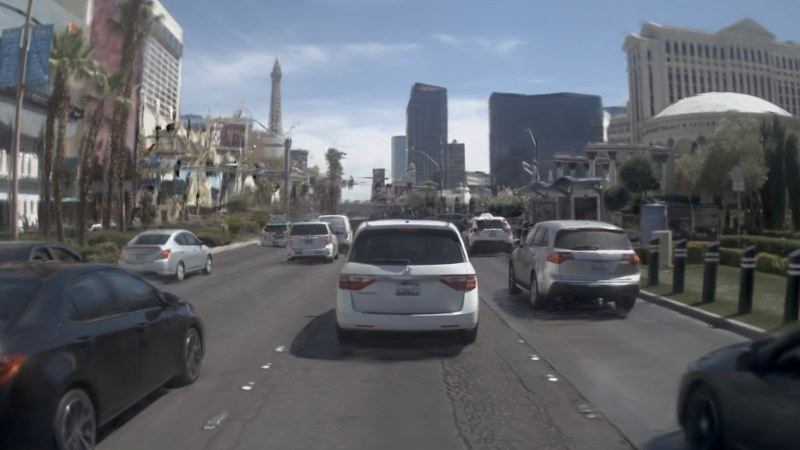
\includegraphics[width=1.9cm]{figures/front_camera_9ad434ec.jpg}};
\node[inner sep=0,draw=white,line width=0.8pt] (cam) at (1.05,-1.80) {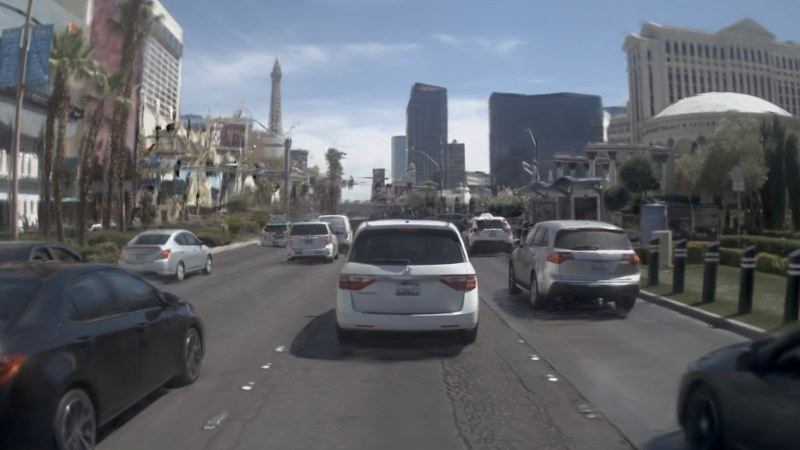
\includegraphics[width=1.9cm]{figures/front_camera_9ad434ec.jpg}};
\node[lab,anchor=south,text=inkC] at (1.13,-1.05) {\small Front camera};
\node[lab,anchor=north] at (1.05,-2.38) {\texttt{PCAM\_F0}: now, $-1$\,s\\352$\times$512};

% encoder, BEV, heads, planner
\node[trapezium,trapezium angle=70,shape border rotate=270,draw=pubB,fill=pubF,minimum height=1.25cm,
      minimum width=1.0cm,align=center,inner sep=1pt] (enc) at (3.25,-1.95) {Vision\\encoder};
\node[lab,anchor=north] at (3.25,-2.62) {ResNet-34};
\draw[pubB,fill=pubF] (4.35,-2.35) rectangle (5.15,-1.55);
\draw[pubB!80,step=0.16] (4.35,-2.35) grid (5.15,-1.55);
\node[lab,anchor=north] at (4.75,-2.4) {latent BEV};
\node[head,minimum width=2.9cm] (heads) at (7.15,-1.42) {Auxiliary heads\\[-1pt]{\scriptsize BEV road map $\cdot$ object boxes}};
\node[pub,minimum width=2.9cm] (plan) at (7.15,-2.5) {Flow-matching planner\\[-1pt]{\scriptsize waypoint flow, 8 steps, $T{=}0$}};

\draw[arr] (cam.east) -- (enc.west);
\draw[arr] (enc.east) -- (4.35,-1.95);
\draw[arr] (5.15,-1.95) -- (5.45,-1.95) |- (heads.west);
\draw[arr] (5.45,-1.95) |- (plan.west);

% inputs below the group
\node[our,text width=3.9cm] (route) at (4.55,-3.85) {Route targets 40/60/80\,m\\[-1pt]{\scriptsize along the route (ours, panel b)}};
\node[pub] (speed) at (8.05,-3.85) {Ego speed};
\coordinate (rin) at (6.75,-3.85);
\draw[arr] (route.east) -- (rin) -- (rin |- plan.south);
\draw[arr] (speed.north) -- (speed.north |- plan.south);

% outputs
\node[pub] (poses) at (9.95,-2.5) {64 poses\\[-1pt]{\scriptsize 0.1\,s apart, 6.4\,s}};
\node[our] (veto) at (11.85,-2.5) {Bend veto\\[-1pt]{\scriptsize ours, panel c}};
\node[sim] (simu) at (13.85,-2.5) {AlpaSim\\[-1pt]{\scriptsize controller}\\[-1pt]{\scriptsize + NuRec render}};
\draw[arr] (plan.east) -- (poses.west);
\draw[arr] (poses.east) -- (veto.west);
\draw[arr] (veto.east) -- (simu.west);
\draw[arr,dashed,draw=headB!90!black] (heads.east) -- (11.85,-1.42) -- (veto.north);
\node[lab,anchor=north] at (10.3,-1.47) {predicted road map,\\object boxes};

% closed loop
\draw[arr,draw=simB!90!black] (simu.north) -- (13.85,-0.25) -- (1.13,-0.25) -- (1.13,-0.7);
\node[lab,anchor=south] at (11.2,-0.25) {rendered frame, ego state, route};

% ---------------------------------------------------------------- (b) route targets
\begin{scope}[shift={(0,-9.25)}]
\node[ttl] at (-0.1,4.55) {(b) Route targets on a bend (every entry from \texttt{lf-009})};
% road band with edges
\draw[line width=19pt,draw=gray!45,line cap=butt] (0.0,0.45) -- (0.6,0.45) arc[start angle=-90,end angle=0,radius=1.34] -- (1.94,4.0);
\draw[line width=17.5pt,draw=gray!10,line cap=butt] (0.0,0.45) -- (0.6,0.45) arc[start angle=-90,end angle=0,radius=1.34] -- (1.94,4.0);
% ego
\draw[fill=routeC!70,draw=routeC] (0.42,0.36) rectangle (0.78,0.54);
\node[lab,anchor=north] at (0.45,0.08) {ego};
% served route
\draw[routeC,line width=0.9pt,densely dotted] (1.94,1.79) -- (1.94,4.0);
\foreach \y in {1.79,2.09,...,3.95} \fill[routeC] (1.94,\y) circle (0.03);
% chord vs arc
\draw[mutedC,dashed,line width=0.6pt] (0.6,0.45) -- (1.94,1.79);
\node[lab,rotate=45,anchor=south] at (1.15,1.02) {straight line};
\node[lab,anchor=north west,text=routeC,align=left] at (1.35,0.15) {42.1\,m along the road\\to the route's start};
% targets: before (hollow, grey) and ours (filled, orange)
\foreach \p in {(1.94,1.895),(1.94,2.895),(1.94,3.895)} \draw[mutedC,line width=0.7pt,fill=white] \p circle (0.075);
\foreach \p in {(1.936,1.685),(1.94,2.685),(1.94,3.685)} \fill[ourB] \p circle (0.075);
\node[font=\scriptsize,anchor=west,text=ourB] at (2.06,1.68) {40};
\node[font=\scriptsize,anchor=west,text=ourB] at (2.06,2.68) {60};
\node[font=\scriptsize,anchor=west,text=ourB] at (2.06,3.68) {80\,m};
\node[lab,anchor=south,text=routeC] at (1.94,4.02) {served route};
% explanation
\node[anchor=north west,text width=4.25cm,font=\scriptsize,align=left] at (2.75,4.05) {%
  {\color{ourB}$\bullet$} \textbf{Ours:} targets at 40/60/80\,m are measured along the road. The served route starts $10\times80/19\approx42.1$\,m ahead; the 40\,m target is extrapolated from the route's initial curvature.\\[3pt]
  {\color{mutedC}$\circ$} \textbf{Before:} the straight-line distance to the route's first point was used as its arc offset, so on a bend every target shifts along the route.\\[3pt]
  We also keep the served route whole rather than cutting it at the point nearest the ego.};
\end{scope}

% ---------------------------------------------------------------- (c) bend veto
\begin{scope}[shift={(7.45,-9.25)}]
\node[ttl] at (-0.1,4.55) {(c) Bend veto (\texttt{lf-013})};
% road band (left bend) with centre line
\draw[line width=21pt,draw=gray!45,line cap=butt] (0.0,0.45) -- (0.4,0.45) arc[start angle=-90,end angle=-5,radius=2.0];
\draw[line width=19.5pt,draw=gray!10,line cap=butt] (0.0,0.45) -- (0.4,0.45) arc[start angle=-90,end angle=-5,radius=2.0];
\draw[gray!55,dashed,line width=0.4pt] (0.0,0.45) -- (0.4,0.45) arc[start angle=-90,end angle=-5,radius=2.0];
% weak predicted road where the nominal plan leaves the road (inside the bend)
\fill[red!55,opacity=0.20] (1.86,1.93) circle (0.36);
\node[lab,text=red!60!black,anchor=east] at (1.42,2.25) {predicted road\\$p<0.5$};
% ego
\draw[fill=routeC!70,draw=routeC] (0.22,0.36) rectangle (0.58,0.54);
\node[lab,anchor=north] at (0.35,0.08) {ego};
% candidate lateral shifts
\foreach \d in {0.14,-0.14,0.28} \draw[mutedC!70,line width=0.5pt,densely dashed,shift={(0,\d)}] (0.58,0.45) arc[start angle=-90,end angle=8,radius=1.32];
% nominal plan (cuts the bend) and accepted shift
\draw[inkC,line width=1.1pt] (0.58,0.45) arc[start angle=-90,end angle=8,radius=1.32];
\draw[ourB,line width=1.6pt,shift={(0,-0.28)}] (0.58,0.45) arc[start angle=-90,end angle=8,radius=1.32];
\node[lab,anchor=south,text=inkC] at (1.95,2.32) {nominal plan};
\node[lab,anchor=west,text=ourB] at (2.4,1.4) {shifted\\plan};
\node[lab,anchor=north west] at (0.95,0.08) {candidate shifts: $\pm0.5$, $\pm1.0$\,m};
% rule
\node[anchor=north west,text width=3.55cm,font=\scriptsize,align=left] at (3.3,4.05) {%
  \textbf{Trigger:} the plan's heading changes by at least $10^\circ$ between 1.0 and 2.5\,s, and the policy's own predicted road probability under the planned footprint is below 0.5.\\[3pt]
  \textbf{Action:} shift the plan laterally by 0.5 or 1.0\,m if the shifted plan is clearly better supported and touches no predicted vehicle; otherwise keep it.\\[3pt]
  \textbf{Local, 1,472 scenes:} acted in 47; 10 off-road zero-score scenes became score one; none lost.};
\end{scope}
\end{tikzpicture}}

\caption{System overview. (a) The \texttt{lf-013} inference loop. The public checkpoint (blue, shaded box) is used unchanged; our changes (orange) are the route-target placement, used by every entry from \lf{} on, and the bend veto, which reads the policy's own predicted road map and object boxes and edits the 64 planned poses before the AlpaSim controller executes them. The camera thumbnail is a frame rendered in one of our local AlpaSim rollouts from the public track assets \cite{trackdata} (CC BY-NC-SA 4.0). (b) Route targets on a bend: we place the 40/60/80\,m targets along the road, using the route's 42.1\,m start offset, where the original adapter used the straight-line distance. (c) Bend veto: the nominal plan cuts a bend where the predicted road is weak, and the veto shifts it laterally. Panels (b) and (c) are schematic and not to scale. Maps and expert futures are absent from the deployed policy interface.}\label{fig:overview}
\end{figure}

We submitted four entries. \lf{} (October 30) is the public checkpoint with the route correction. \texttt{lf-010} (November 6) adds a decoder-only adaptation on SimScale recovery data, plan sampling and a lead-departure rule. \texttt{lf-012} (November 13) returns to \lf{}'s weights and applies the lead-departure rule and a 5$^\circ$ bend veto. \texttt{lf-013} (November 17), our final entry, is the \texttt{lf-012} image with the lead-departure rule switched off and the veto threshold raised to 10$^\circ$, so it is \lf{} plus the bend veto alone. Official results throughout are from the public leaderboard saved on November 18, 2026, after the nuPlan submission deadline.

\section{Policy description}
\subsection{Base policy}\label{sec:base}
The released roughly 68M-parameter Latent TransFuser (LTF) \cite{transfuser} uses a ResNet-34 visual backbone, latent bird's-eye-view features, auxiliary semantic/object heads, and a waypoint-only flow planner. For nuPlan it consumes \texttt{PCAM\_F0} (packaged at width 352, height 512), its one-second history frame, ego speed, and up to three route targets. The planner produces 64 ego-frame poses at 0.1 s spacing, using eight flow integration steps and zero sampling temperature for the nominal plan. The adapter supplies positions and headings; the simulator's controller produces steering and acceleration. The predicted road map and object boxes used by the rules below are model output, not privileged ground truth.

\subsection{Route-interface correction}\label{sec:route}
The served route begins ahead of the ego. Treating the straight distance to its first point as route arc length misplaces the checkpoint's 40/60/80 m targets on bends. Our adapter uses the pinned runtime's route-start arc offset ($10\times80/19\simeq42.105$ m), interpolates along the supplied polyline, and estimates the short missing segment for the 40 m target from its initial curvature. It retains the original construction when the expected spacing check fails; this heuristic is specific to that route contract. A second switch keeps the served route intact instead of truncating it at the point nearest the ego, which could remove targets on tight turns. Neither correction reads an HD map, future logged trajectory, or scene identity at deployment. Every entry from \lf{} on uses both switches.

\subsection{Bend veto}\label{sec:veto}
The bend veto is the only rule in our final entry. When the nominal plan bends by at least 10$^\circ$ and the policy's own predicted road map gives probability below 0.5 under the planned footprint, the plan is shifted laterally by 0.5 or 1.0 m if the shifted plan is clearly better supported and touches no predicted vehicle; otherwise the plan is kept. The veto changes only the path, never the timing along it. \texttt{lf-012} ran the same rule with a 5$^\circ$ threshold alongside the lead-departure rule below; \texttt{lf-013} is the \texttt{lf-012} image with two settings changed and no file changed: the lead-departure rule is switched off and the bend threshold is raised to 10$^\circ$. We chose this configuration because, on all 1,472 local scenes, the stand-alone veto acted in 47 scenes, turned 10 off-road zero-score scenes into score-one scenes, and lost no score-one scene.

\subsection{Earlier inference variants}\label{sec:variants}
\texttt{lf-010} includes \emph{Track A}, which samples 16 plans at temperatures 1.5/2.0 and switches only when the nominal plan fails checks using predicted road and object outputs. It then applies a \emph{lead-departure rule}: for ego speed below 0.5 m/s, a predicted moving lead and existing motion intent, it accelerates progress along the nominal path subject to gap and predicted-box checks. The implementation can extrapolate beyond the nominal path. These two rules and the changed weights were submitted together, so the official result does not identify which component caused \texttt{lf-010}'s regression. \texttt{lf-012} keeps \lf{}'s weights, uses no sampling, and applies the lead-departure rule together with the 5$^\circ$ bend veto. Which of \texttt{lf-012}'s two rules cost it PCS could not be resolved from local data, which is why the final entry removed the lead-departure rule and kept the veto.

\section{Resources and training}
\subsection{Public resources and licenses}
Table~\ref{tab:resources} lists every external resource. The base checkpoint's card additionally discloses Physical AI AV and NuRec pretraining, governed by the NVIDIA Autonomous Vehicle Dataset License \cite{nvidiadata}; we inherit these weights rather than repeat that training. No private dataset was added by our team. SimScale's code is Apache-2.0; its data license is distinct.

\begin{table}[htbp]
\centering\small
\caption{Public resources and declared terms. Links are in the references.}\label{tab:resources}
\begin{tabular}{L{3.0cm}L{5.0cm}L{3.8cm}}
\toprule
Resource & Use & License / terms \\
\midrule
py123d\_garage / 123D & Policy, driver, conversion tools \cite{garage,py123d} & Apache-2.0 code \\
Released waypoint seed 1 & Unchanged \lf{} initialization \cite{weights} & CC BY-NC-SA 4.0 \\
nuPlan / OpenScene & Real observations, poses, boxes, routes \cite{nuplan,openscene} & CC BY-NC-SA 4.0; nuPlan terms \\
SimScale recovery & Synthetic observations/labels \cite{simscale} & CC BY-NC-SA 4.0 data \\
AlpaSim / track assets & Simulation; later research collection \cite{alpasim,trackdata} & Apache-2.0 code; CC BY-NC-SA 4.0 assets \\
\bottomrule
\end{tabular}
\end{table}

\subsection{Decoder-only adaptation for \texttt{lf-010}}\label{sec:lf010}
We start from the same public seed-1 weights and update only the planning decoder. The corrected SimScale recovery corpus supplies perturbed observations and four-second targets. We repaired timestamp/route conversion, excluded invented future tails from supervised labels, and paired opposite teacher-relative lateral residuals within city, turn and speed groups. The retained training pools contain 3,412 recovery and 2,272 rendered-preservation anchors, plus 512 independent real-image preservation examples. All 44 public-evaluation source recordings and eight reserved recordings are excluded from this recovery training pool.

The submitted checkpoint uses 1,024 AdamW steps, batch 4, float32, learning rate $5\times10^{-6}$, zero weight decay and gradient clipping at 1. Batch shares are 25\% recovery, 12.5\% rendered preservation and 62.5\% real preservation. Four-second supervision uses the first 40 poses; detached teacher continuation fills the remaining horizon before noising. On preservation examples we match the frozen \lf{} teacher's denoising output. City quotas prevent the large Las Vegas pool from dominating. This schedule visits 1,024 distinct recovery anchors; ``full pool'' describes selection coverage, not a full training epoch. Appendix~\ref{app:detail} gives the per-city exposure.

\subsection{On-policy adaptation, not submitted}\label{sec:onpolicy}
Inspired by RoaD \cite{road}, we collect guided public-development rollouts using 64 policy samples and logged-human trajectory guidance, then fit only the flow denoiser while preserving the original policy on normal observations. Maps and human futures are collection-only inputs. These experiments use 14,624,767 trainable parameters, cached frozen features, float32 AdamW, learning rate $5\times10^{-6}$, batch 8 and 256 steps; their mixture is 25\% recovery, 25\% rendered preservation and 50\% real preservation. This differs from the submitted SimScale recipe. Public recordings used for collection are retired from validation for this branch; prior public-set reuse is still disclosed. Section~\ref{sec:onpolicyresults} reports the outcome.

\section{Results}\label{sec:results}
\subsection{Local protocol}
Our local benchmark uses AlpaSim with the public nuPlan/MTGS assets. The public manifest contains 1,485 scenes; the matched comparison below covers 1,472 available/scored scenes across 44 recordings, and we retain the evaluated scene IDs. Local runs use 2 Hz replanning after 0.5 s initial takeover, the pinned scorer with its corridor correction, and fixed controller gains. We compare identical scene lists, repair a non-reproducing historical baseline batch with a fresh baseline, and report score changes together with incidents and score-one retention. The 609-scene development panel overrepresents hard scenes, so its weighted estimate is kept apart from the unweighted 1,472-scene mean; the complementary 863 scenes assess regressions on easier cases. Section~\ref{sec:limits} discusses how far this proxy stands from the private official suite.

\subsection{Local comparison}
Table~\ref{tab:local} gives the corrected local comparison. The bend-veto-only row is \texttt{lf-013}'s rule run stand-alone on November 11; with official-mix scene weights its gain over \lf{} is $+0.0086$ [$+0.0029$, $+0.0154$]. Lead-only is a local experiment, not a separate official entry. On this benchmark every variant beats \lf{}, and every combined-rule variant beats the veto alone.

\begin{table}[htbp]
\centering\small
\caption{Corrected local comparison on 1,472 matched scenes. Zeros are scenes with exactly zero score; incidents are scenes with an off-road event or an at-fault collision.}\label{tab:local}
\begin{tabular}{lrrr}
\toprule
Variant & Mean score $\uparrow$ & Zero scenes $\downarrow$ & Incidents $\downarrow$ \\
\midrule
\lf{} & 0.9132 & 52 & 52 \\
\lf{} + lead rule only & 0.9189 & 52 & 52 \\
SimScale-512 + both rules & 0.9272 & 41 & 40 \\
SimScale-1024 + both rules (\texttt{lf-010}) & 0.9303 & 38 & 38 \\
\lf{} + lead rule + 5$^\circ$ bend veto (\texttt{lf-012}) & 0.9277 & 39 & 39 \\
\lf{} + 10$^\circ$ bend veto only (\texttt{lf-013}) & 0.9200 & 42 & 42 \\
\bottomrule
\end{tabular}
\end{table}

\subsection{Official results}\label{sec:official}
Table~\ref{tab:official} gives all four entries from one public leaderboard snapshot \cite{board}, saved on November 18, 2026 at 18:56 IST after the submission deadline, with 286 entries from 63 accounts: 57 participating teams and six host accounts. PCS is jointly fitted and changes with the reference population; in the November 13 snapshot \lf{}, \texttt{lf-010} and \texttt{lf-012} had PCS 2302, 2240 and 2261. The bracketed ranges are the board's 95\% posterior intervals from its jointly fitted model, whereas the local means in Table~\ref{tab:local} are point estimates over the 1,472 scenes. Among the participating teams' best entries, \texttt{lf-013}'s PCS is the 4th highest of 57. The board's own rank column orders entries by a conservative rank bound and lists \lf{} 13th and \texttt{lf-013} 21st of 286 entries. Late-evaluated entries kept arriving after this snapshot, and every arrival refits all scores: on November 18 at 20:11 IST (291 entries) \texttt{lf-013} had PCS 2528 and our team was 4th in both orderings. Final standings follow the organizers' additional evaluation runs for the top teams.

\begin{table}[htbp]
\centering\small
\caption{Official nuPlan results of all four entries, from the public leaderboard snapshot of November 18, 2026 (18:56 IST, 286 entries) \cite{board}. Brackets are the board's 95\% posterior intervals.}\label{tab:official}
\begin{tabular}{lrrr}
\toprule
Entry & Mean score $\uparrow$ & PCS [95\% interval] $\uparrow$ & km / incident $\uparrow$ \\
\midrule
\lf{} & 0.9454 & 2487 [2341, 2633] & 1.039 \\
\texttt{lf-010} & 0.9433 & 2367 [2218, 2515] & 0.929 \\
\texttt{lf-012} & 0.9462 & 2412 [2250, 2574] & 1.110 \\
\texttt{lf-013} & 0.9494 & 2502 [2317, 2687] & 1.364 \\
\bottomrule
\end{tabular}
\end{table}

Figure~\ref{fig:position} tracks our position over the challenge by each team's best PCS so far. Every point uses the scores refitted on the post-deadline board of November 18, so earlier positions can differ from what the board showed on that day. Our line ends 4th of the 57 participating teams; the board's rank column places our team 9th in the same snapshot and 4th in the later refit above.

\begin{figure}[htbp]
\centering
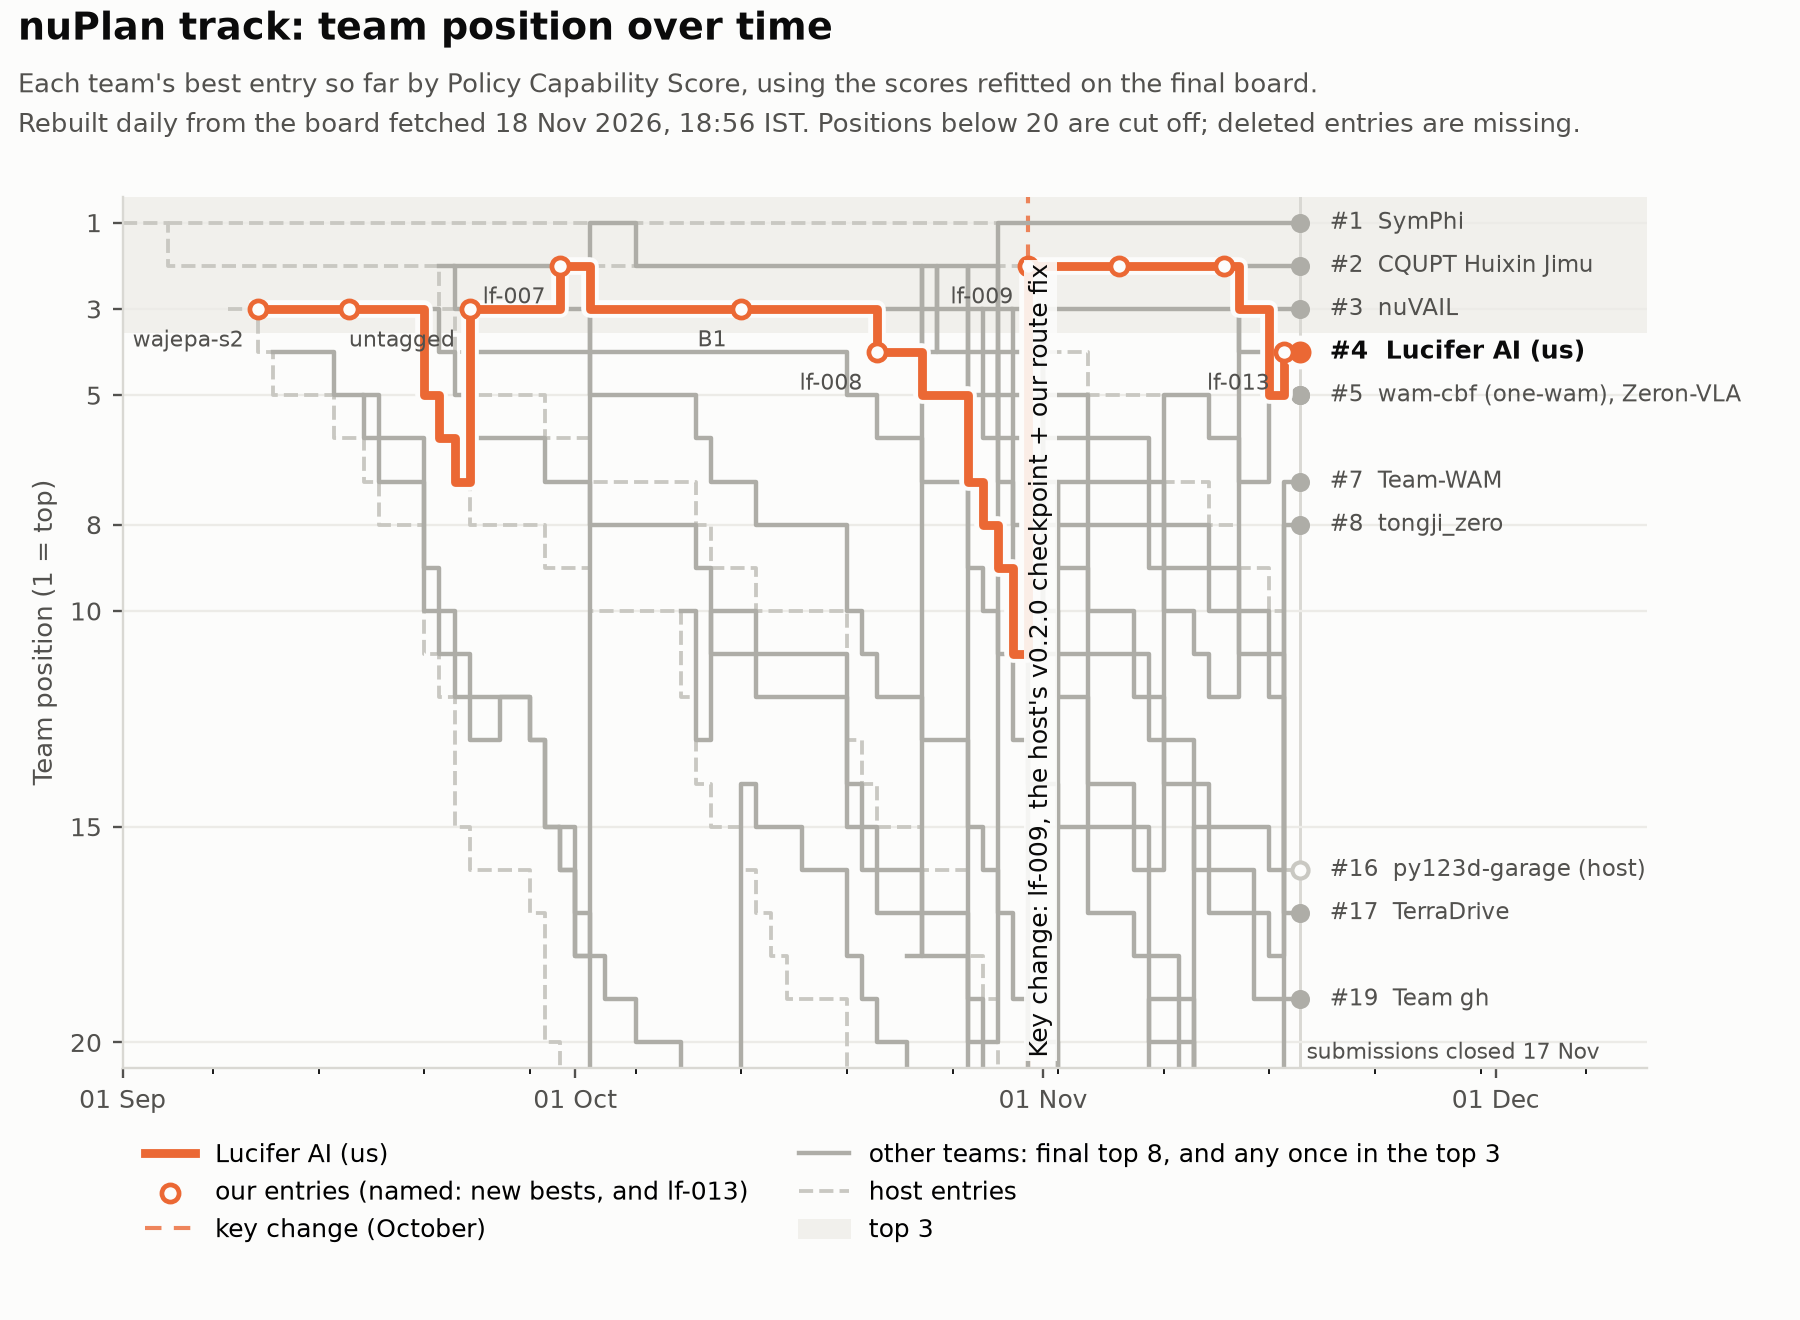
\includegraphics[width=\linewidth]{figures/nuplan-team-position-20261118.png}
\caption{Team position over time on the nuPlan public board, by each team's best PCS so far, using the scores refitted on the post-deadline board of November 18. The vertical line marks \lf{}, the host's v0.2.0 checkpoint with our route fix. Positions below 20 are cut off.}\label{fig:position}
\end{figure}

\subsection{What transferred}\label{sec:transfer}
On the earlier 1,473-scene matched panel, exact arc targets increased the mean by 0.0054 and reduced zero-score scenes from 62 to 52. At the October 31 official snapshot, \lf{} scored 0.9454 versus 0.9437 for the host's entry using the same released checkpoint. In contrast, \texttt{lf-010}'s local gain of about 0.017 did not transfer: its official mean decreased by 0.00217 and incident distance worsened. \texttt{lf-012}, which changes no weights, shows a different failure: its official mean rose by 0.00072 and its incident distance improved, yet its PCS point estimate is 75 below \lf{}'s. \texttt{lf-013}, the smallest change, is the only variant that carried over on all three measures: its official mean rose by 0.0040, its distance between at-fault incidents by 31\% (1.039 to 1.364 km), and its PCS point estimate by 15. The two rule entries also differ in footprint. \texttt{lf-012}'s distance to the human path rose 3.0\% officially (0.585 to 0.603 m) against 1.5\% locally, so its rules acted more, or moved more, on the hidden recordings; \texttt{lf-013}'s rose 0.7\% officially against 0.9\% locally. The PCS intervals of all four entries overlap (Section~\ref{sec:limits}).

\subsection{Why mean score is insufficient}
The organizer's Drive-IRT implementation models zero, intermediate and score-one outcomes separately \cite{driveirt}. We also count transitions at its 0.0001/0.9999 cutoffs; its zero class includes near-zero progress scores beyond Table~\ref{tab:local}'s exact zeros. \texttt{lf-010} loses 11 locally score-one scenes; lead-only loses none and improves 32 scene scores without worsening any. However, local PCS still ranks \texttt{lf-010} above \lf{}. Thus neither the mean nor this local PCS fit explains the official reversal. \texttt{lf-012} was selected to lose no local score-one scene (it gains 21 and removes 13 incident scenes), yet its PCS is also below \lf{}'s. The stand-alone veto in \texttt{lf-013} acts in fewer scenes, changes only the path, and passed the same local test (10 gained, none lost); it is the one rule whose local signal transferred.

\subsection{On-policy adaptation}\label{sec:onpolicyresults}
Table~\ref{tab:onpolicy} compares the on-policy branch of Section~\ref{sec:onpolicy} with a fresh \lf{} on 48 preselected public scenes. Neither round's interval excludes zero. Larger gains on a repeatedly used 11-scene development panel are dominated by one Pittsburgh stall rescue, and the broader comparison does not establish general improvement. A separate earlier-intervention \emph{teacher}, used only at collection time, reduces off-road failures from 6 to 3 on 24 training scenes, with score 0.750 to 0.875 and no lost perfect control; its three rescues span only two recordings, and wrong-lane flags increase from 9 to 10. Later guided and shadow-label fits, including the failed 417-scene development check, are recorded in Appendix~\ref{app:history}.

\begin{table}[htbp]
\centering\small
\caption{Unguided learned-policy comparison on 48 preselected public scenes (20 recordings; 12 scenes per city). Intervals bootstrap recordings. No arm loses a score-one scene or adds a scored hard failure on this panel.}\label{tab:onpolicy}
\begin{tabular}{lrr}
\toprule
Policy & Mean score & Paired gain [95\% interval] \\
\midrule
Fresh \lf{} & 0.86835 & --- \\
On-policy round 1, step 256 & 0.87081 & +0.00246 [$-0.00020$, +0.00840] \\
On-policy round 2, step 256 & 0.87010 & +0.00174 [$-0.00004$, +0.00481] \\
\bottomrule
\end{tabular}
\end{table}

\section{Runtime and reproducibility}
\paragraph{Compute.}
Local adaptation/evaluation used one NVIDIA RTX PRO 4000 Blackwell GPU with 24 GB VRAM. One local evaluation of all 1,472 public scenes took about 3.5--3.7 hours on this GPU. Full-model training of the older checkpoint ran at about 190 samples per second, for example about 2 hours for seven epochs on 184,612 training samples; cached features permit much shorter decoder-only runs. We did not log total GPU hours. The whole project, including the experiment families in Appendix~\ref{app:history}, used substantially more compute than the runs reported in the main text.

\paragraph{Latency.}
In the combined-rule local run, additional sampling averaged 26.8 ms per call over 6,090 calls, on top of approximately 33 ms nominal inference. These are local component timings: they exclude parts of the simulator/RPC pipeline and are neither official end-to-end latency nor a peak-VRAM measurement.

\paragraph{Entries and artifacts.}
All four entries completed successfully, and every warm-up scored 32/32 rollouts. Because of the deadline, \texttt{lf-013}'s official submission was sent while its warm-up was still queued; the warm-up ran and succeeded afterwards. Appendix~\ref{app:repro} records the submission identities, checkpoint hashes and container digests of all four entries, and the exact leaderboard responses behind Table~\ref{tab:official}.

\section{Limitations and safety considerations}\label{sec:limits}
\paragraph{Validity of the local benchmark.}
Our local benchmark is a public proxy, not a reproduction of the private 1,000-rollout official suite; runtime and replanning differences add to the transfer uncertainty. Repeated model selection on the same public recordings limits the independence of the local results. The \lf{} comparison with the host's entry is an observed entry comparison, not a controlled official ablation of every runtime detail.

\paragraph{Statistical resolution.}
\texttt{lf-013} has our best official point estimates, but its PCS interval overlaps \lf{}'s, and the intervals of all four entries overlap; we treat the entries as statistically indistinguishable on the public board and claim no resolved capability difference from the point estimates. We make no fixed ``PCS per mean-score point'' conversion, and we do not claim that the private nuPlan set is out of distribution. A single entry cannot show whether the lead rule or the 5$^\circ$ threshold caused \texttt{lf-012}'s loss. The earlier-intervention teacher of Section~\ref{sec:onpolicyresults} is a collection-time tool, not a learned checkpoint or a leaderboard result.

\paragraph{Failure modes.}
Off-road drift and incomplete progress remain material weaknesses. Sparse look-ahead route points provide no direct near-field road guarantee; predicted BEV boundaries and object velocities can be inaccurate. Lead-only changed motion during recorded human-wait intervals in four scenes despite tied scene scores; it has no traffic-light input or reliable lane-level lead association. A 70-scene targeted guard study reduced gains with motion/path-support vetoes, while a collision veto was inactive. Zero new scored incidents therefore does not demonstrate safe waiting behavior or safe extrapolation. In six inspected stall rollouts the rendered traffic lights never changed, and one apparent red signal was a light on a building facade (Figure~\ref{fig:signal}); we built no rule that departs at a rendered red light.

\paragraph{Safety and broader impact.}
All results are simulation evidence. A score of one can reflect saturated progress rather than flawless driving; unscored behaviors still matter. Shared recordings, repeated selections, short rollouts, limited recovery labels and private/public differences constrain generalization. The bend veto and the lead-departure rule are tuned to one simulator and one route format, have no traffic-light input, and are research findings, not safety mechanisms or validated real-vehicle behavior. The positive contribution of this work is methodological: it records which local improvements did and did not transfer to a hidden closed-loop benchmark, which may help others avoid over-trusting public-scene scores. We release no model or data.

\section{Conclusion}
Four entries built on one public checkpoint gave a clear ordering on the hidden benchmark that our local benchmark did not predict. The two changes that transferred, the route-interface correction and the bend veto, each touch an interface of the policy and use only its inputs and its own predictions. The changes that did not transfer, a decoder-only adaptation on synthetic recovery data, plan sampling and a lead-departure rule, raised the local mean score and lowered official PCS. With all PCS intervals overlapping, the safe reading is narrow: on this benchmark, small inference-side corrections grounded in the policy's own perception carried over, and local gains from larger changes did not. The experiment history in Appendix~\ref{app:history} and the artifact identities in Appendix~\ref{app:repro} are provided so that both findings can be checked.

\section*{Acknowledgements}
We thank the AlpaSim challenge organizers at NVIDIA, KE:SAI and HKU (OpenDriveLab), and the py123d\_garage team for the public baseline we built on. AI coding and writing assistants were used for implementation, analysis and drafting; the author checked all results and references.

\begin{thebibliography}{99}
\bibitem{garage} KE:SAI Labs. \emph{py123d\_garage}, code and AlpaSim adapter. \url{https://github.com/kesai-labs/py123d_garage}. Pinned entry code: v0.2.2, \texttt{ad6cb51}, plus our route patch.
\bibitem{weights} KE:SAI Labs. \emph{py123d\_garage pretrained checkpoints}, file \texttt{v0.2.0/ltf-base-waypoints-68M/posttrain/model\_1.pth}. \url{https://huggingface.co/kesai-labs/py123d_garage_pretrained_checkpoints}.
\bibitem{py123d} D. Dauner et al. \emph{123D: Unifying Multi-Modal Autonomous Driving Data at Scale}. arXiv:2605.08084, 2026. \url{https://arxiv.org/abs/2605.08084}.
\bibitem{nuplan} Motional. \emph{nuPlan dataset and terms of use}. \url{https://www.nuscenes.org/nuplan}; \url{https://www.nuscenes.org/terms-of-use}.
\bibitem{openscene} OpenDriveLab. \emph{OpenScene sensor data}. \url{https://huggingface.co/datasets/OpenDriveLab/OpenScene}.
\bibitem{simscale} H. Tian et al. \emph{SimScale: Learning to Drive via Real-World Simulation at Scale}. arXiv:2511.23369, 2025. \url{https://huggingface.co/datasets/OpenDriveLab/SimScale}.
\bibitem{alpasim} NVIDIA. \emph{AlpaSim}. \url{https://github.com/NVlabs/alpasim}.
\bibitem{trackdata} OpenDriveLab. \emph{AlpaSim Challenge 2026 nuPlan track assets}. \url{https://huggingface.co/datasets/OpenDriveLab/AlpasimChallenge2026_nuplan_track}.
\bibitem{driveirt} KE:SAI Labs. \emph{Drive-IRT}. \url{https://github.com/kesai-labs/drive-irt}. Reviewed implementation: \texttt{82ddd5a42333cacf94c3b652d531101484567f47}.
\bibitem{road} G. Garcia-Cobo et al. \emph{RoaD: Rollouts as Demonstrations for Closed-Loop Supervised Fine-Tuning of Autonomous Driving Policies}. arXiv:2512.01993, 2025. \url{https://arxiv.org/abs/2512.01993}.
\bibitem{nvidiadata} NVIDIA. \emph{Physical AI Autonomous Vehicles and NuRec}. \url{https://huggingface.co/datasets/nvidia/PhysicalAI-Autonomous-Vehicles}; \url{https://huggingface.co/datasets/nvidia/PhysicalAI-Autonomous-Vehicles-NuRec}. The inherited checkpoint card identifies these resources and the NVIDIA Autonomous Vehicle Dataset License.
\bibitem{board} NVIDIA. \emph{AlpaSim E2E Closed Loop Challenge 2026 leaderboard}. \url{https://nvidia-alpasime2eclosedloopchallenge2026.hf.space/}. Official results use saved dated responses, not a live ranking.
\bibitem{gatedvla} K. Hiratsuka, N. Takada and M. Kawano. \emph{GatedVLA with Camera-Based Emergency Braking: AlpaSim E2E Closed Loop Challenge Technical Report}. arXiv:2611.01663, 2026.
\bibitem{laosiji} C. Gao et al. \emph{Lao Siji: Adapting openpilot to Closed-Loop End-to-End Driving in Neural Reconstruction}. arXiv:2611.19922, 2026.
% References below support Appendix C. arXiv identifiers, titles and first authors were checked against the arXiv API,
% and every URL returned HTTP 200, on 2026-11-09.
\bibitem{vavam} F. Bartoccioni et al. \emph{VaViM and VaVAM: Autonomous Driving through Video Generative Modeling}. arXiv:2502.15672, 2025. Code: \url{https://github.com/valeoai/VideoActionModel}.
\bibitem{mup} G. Yang et al. \emph{Tensor Programs V: Tuning Large Neural Networks via Zero-Shot Hyperparameter Transfer}. arXiv:2203.03466, 2022.
\bibitem{wajepa} X. Wang et al. \emph{WA-JEPA: Rethinking the Video JEPA Paradigm for World-Action Modeling in Autonomous Driving}. arXiv:2608.20974, 2026. Checkpoints: \url{https://huggingface.co/AFARI-Research/WA-JEPA}.
\bibitem{gtrs} Z. Li et al. \emph{Generalized Trajectory Scoring for End-to-end Multimodal Planning}. arXiv:2506.06664, 2025. Code: \url{https://github.com/NVlabs/GTRS}.
\bibitem{cosmos3edge} NVIDIA. \emph{Cosmos3-Edge} model card. \url{https://huggingface.co/nvidia/Cosmos3-Edge}.
\bibitem{cosmos} NVIDIA. \emph{Cosmos World Foundation Model Platform for Physical AI}. arXiv:2501.03575, 2025.
\bibitem{odyssey} Odyssey. \emph{Introducing Odyssey-3: A General-Purpose Physical Intelligence}. Announcement, \url{https://odyssey.systems/introducing-odyssey-3}.
\bibitem{optuna} T. Akiba et al. \emph{Optuna: A Next-generation Hyperparameter Optimization Framework}. arXiv:1907.10902, 2019.
\bibitem{transfuser} K. Chitta et al. \emph{TransFuser: Imitation with Transformer-Based Sensor Fusion for Autonomous Driving}. arXiv:2205.15997, 2022.
\bibitem{pdm} D. Dauner et al. \emph{Parting with Misconceptions about Learning-based Vehicle Motion Planning}. arXiv:2306.07962, 2023.
\bibitem{hydramdp} Z. Li et al. \emph{Hydra-MDP: End-to-end Multimodal Planning with Multi-target Hydra-Distillation}. arXiv:2406.06978, 2024.
\bibitem{wiseft} M. Wortsman et al. \emph{Robust fine-tuning of zero-shot models}. arXiv:2109.01903, 2021.
\bibitem{soups} M. Wortsman et al. \emph{Model soups: averaging weights of multiple fine-tuned models improves accuracy without increasing inference time}. arXiv:2203.05482, 2022.
\bibitem{dagger} S. Ross, G. J. Gordon and J. A. Bagnell. \emph{A Reduction of Imitation Learning and Structured Prediction to No-Regret Online Learning}. arXiv:1011.0686, 2010.
\bibitem{rogdagger} L. Zhong et al. \emph{RoG-DAgger: Rollout-Guided Post-Training for End-to-End Driving}. arXiv:2608.24525, 2026.
\bibitem{lead} L. Nguyen et al. \emph{LEAD: Minimizing Learner-Expert Asymmetry in End-to-End Driving}. arXiv:2512.20563, 2025.
\bibitem{nuscenes} H. Caesar et al. \emph{nuScenes: A multimodal dataset for autonomous driving}. arXiv:1903.11027, 2019.
\bibitem{nureasoning} \emph{nuReasoning} dataset. \url{https://huggingface.co/datasets/nureasoning/nuReasoning}.
\bibitem{drivecot} T. Wang et al. \emph{DriveCoT: Integrating Chain-of-Thought Reasoning with End-to-End Driving}. arXiv:2403.16996, 2024.
\bibitem{cascade} NVIDIA. \emph{CASCADE: Causal Spatio-Temporal Analysis of Driving Environments} dataset. \url{https://huggingface.co/datasets/nvidia/cascade}.
\bibitem{worldengine} OpenDriveLab. \emph{WorldEngine} dataset. \url{https://huggingface.co/datasets/OpenDriveLab/WorldEngine}.
\bibitem{diffplanner} Y. Zheng et al. \emph{Diffusion-Based Planning for Autonomous Driving with Flexible Guidance}. arXiv:2501.15564, 2025. Code: \url{https://github.com/ZhengYinan-AIR/Diffusion-Planner}.
\bibitem{hdp} Y. Zheng et al. \emph{Unleashing the Potential of Diffusion Models for End-to-End Autonomous Driving}. arXiv:2602.22801, 2026. Code (Hyper-Diffusion-Planner): \url{https://github.com/ZhengYinan-AIR/Hyper-Diffusion-Planner}.
\bibitem{diffusiondrive} B. Liao et al. \emph{DiffusionDrive: Truncated Diffusion Model for End-to-End Autonomous Driving}. arXiv:2411.15139, 2024.
\bibitem{wamflow} Y. Xu et al. \emph{WAM-Flow: Parallel Coarse-to-Fine Motion Planning via Discrete Flow Matching for Autonomous Driving}. arXiv:2512.06112, 2025. Code: \url{https://github.com/fudan-generative-vision/WAM-Flow}.
\bibitem{alpamayo} NVIDIA. \emph{Alpamayo-R1: Bridging Reasoning and Action Prediction for Generalizable Autonomous Driving in the Long Tail}. arXiv:2511.00088, 2025.
\bibitem{opted} D. Da Col et al. \emph{OPTED: On-Policy Fine-Tuning for End-to-End Driving using a Render-Free Teacher}. arXiv:2609.20756, 2026.
\end{thebibliography}

\appendix
\section{Artifact identities and reproducibility}\label{app:repro}
\paragraph{Primary entry.}
\lf{} is submission \nolinkurl{bcb5aca3-6b1d-4a72-8b3c-780dffd5ab03}. The upstream seed-1 file is packaged as \texttt{/opt/checkpoint/model\_0.pth}; that filename change does not change the seed or weights. Its SHA-256 is \nolinkurl{ae1619d546e5aacfa7540b2b5edbcdf49b2f321b7fccd94374452eded243aaca}. The registry manifest digest is \nolinkurl{sha256:c84c50b819e33cce16cd2ed06c44145a0e85d3668cf78a37a322220f6d649ec1}. The image enables \texttt{exact\_route\_targets=true} and \texttt{keep\_served\_route\_whole=true}; default controller gains are unchanged.

\paragraph{Adapted entry.}
\texttt{lf-010} is submission \nolinkurl{d8218a87-2f75-41e7-bbb6-9329ae37a63e}, registry manifest \nolinkurl{sha256:11ac326e736096d71a3c61f7b0072b360df37c9d5f6e2275ac5221b423775188}. It replaces only the checkpoint in the combined-hook image. Its recipe is the 1,024-step corrected recovery run, not the earlier uncorrected step-500 run, the later 3,412-step extension, or the on-policy experiment. It uses the same underlying route fixes. Local Docker image IDs and registry manifest digests are tracked separately; they are not interchangeable identities.

\paragraph{Rule-only entry.}
\texttt{lf-012} is submission \nolinkurl{346b9928-1884-40a0-b9eb-5c7fbd797b5c}, registry manifest \nolinkurl{sha256:571f5691ab78cbfe2b440e93da883ebe41062fe7524727d4320cc0ab9148a4f2}. It adds a rule layer to the \lf{} image: the checkpoint, driver files and route fixes are byte-identical to \lf{}, the lead-rule file is identical to \texttt{lf-010}'s, and the bend limit is 5$^\circ$. Follow-through, adjacent-traffic and fallback code paths in that layer are switched off and did not run. Default controller gains are unchanged.

\paragraph{Final entry.}
\texttt{lf-013} is submission \nolinkurl{81976c46-e9f8-453e-a7d2-06902c53b8b8}, registry manifest \nolinkurl{sha256:82147ba3889e8c105e7e075e1dd14c1f5bee8dbdbfa421d2dc367136a3836084}. Its Dockerfile builds from the \texttt{lf-012} image (manifest \nolinkurl{sha256:571f5691ab78cbfe2b440e93da883ebe41062fe7524727d4320cc0ab9148a4f2}) and sets only \texttt{LEAD\_ARM=off} and \texttt{VETO\_BEND\_DEG=10}; no file changes. The image's startup line reports \texttt{veto=active lead=off adjacent=off bend\_deg=10.0}. The rule files match, by SHA-256, those of the November 11 stand-alone veto run, and the veto reproduces that run's decisions on all 770 saved planning calls offline; equivalence was shown offline, not by a new closed-loop run. The stand-alone run's per-scene results are retained in the author's records.

\paragraph{Official snapshot and local denominator.}
Table~\ref{tab:official} and Table~\ref{tab:entries} use a saved leaderboard response fetched 2026-11-18 18:56:59 IST, after the November 16 (AoE) submission deadline, i.e.\ 11:59 UTC on November 17, with 286 entries from 63 accounts (57 participating teams and six host accounts). The November 13 values quoted in Section~\ref{sec:official} come from a response saved 2026-11-13 11:05:41 IST with 244 entries. Table~\ref{tab:local} uses the corrected 609+863 comparison, not the old non-reproducing baseline or a weighted 331-scene extrapolation. Its \texttt{lf-012} row comes from a later run of the same 1,472 scenes, executed as 814 development and 658 confirmation scenes and compared scene by scene with the same \lf{} scores. The earlier route-interface ablation has 1,473 scenes and is reported separately. No absent scene is silently imputed a perfect score. The saved leaderboard responses and per-scene metric artifacts are available from the author on request.

\section{Additional experimental detail}\label{app:detail}
\paragraph{Recovery exposure.}
The retained 3,412 training anchors comprise Las Vegas 2,168, Boston 604, Pittsburgh 322 and Singapore 318. The 1,024 supervised draws visit 448, 232, 176 and 168 distinct anchors in those cities, respectively. Rendered controls contribute 512 distinct draws; the 512 real controls contribute 2,560 draws. On reused reserved examples, recovery error improves by 0.1667 m at step 512 and 0.2719 m at step 1,024. Real-image deviation from \lf{} is respectively 0.0356 and 0.0509 m; these are teacher-relative deviations, not accuracy against human labels. These open-loop checks did not predict official transfer.

\paragraph{On-policy data separation.}
The later collection branch splits the 44 public recordings into 22 development and 22 protected confirmation recordings; development is further divided into 12 collection and 10 selection recordings. The first expanded training pool contains 541 recovery and 556 rendered-preservation anchors plus 512 real controls outside the 44 public logs. Round 2 adds 182 recovery anchors. A separate startup-coverage arm reconstructs actual warm-up poses instead of mistaking shadow controller predictions for executed motion. It adds 137 recovery and 155 rendered controls, but does not improve the reused development result. Native initial history is padded when real history is unavailable; it is not described as an observed one-second past frame.

The 48-scene panel is preselected for the compared learned arms, but uses public recordings with historical exposure. Singapore has no open-loop selection recording in this branch, although it is represented in closed-loop panels. These limits preclude a strong claim of independent distributional validation. Neither public collection guidance nor map/label checks are available to the submitted inference policy. The author's records index supporting files and hashes, separating observations from proposals, and are available on request.

\paragraph{Rendered traffic lights.}
For 6 of the 20 local stall rollouts that we had labelled ``held at a signal, no lead, no cue'', we extracted the rendered front-camera frames 0.5, 3.5 and 5.0 s after takeover. In all six the rendered signals look the same at the three times, although the logged human driver departed 0.8--3.0 s after takeover: clearly red in three, ambiguous in three. Figure~\ref{fig:signal} shows one ambiguous case, in which what reads as a red signal is a glow on a building facade while the real signal heads are ghosted by the reconstruction. A static scene reconstruction cannot show a light change, so these stalls do not show that the policy ignores a green light, and departure fine-tuning on nuPlan frames cannot remove them. We inspected only six rollouts, by eye.

\begin{figure}[htbp]
\centering
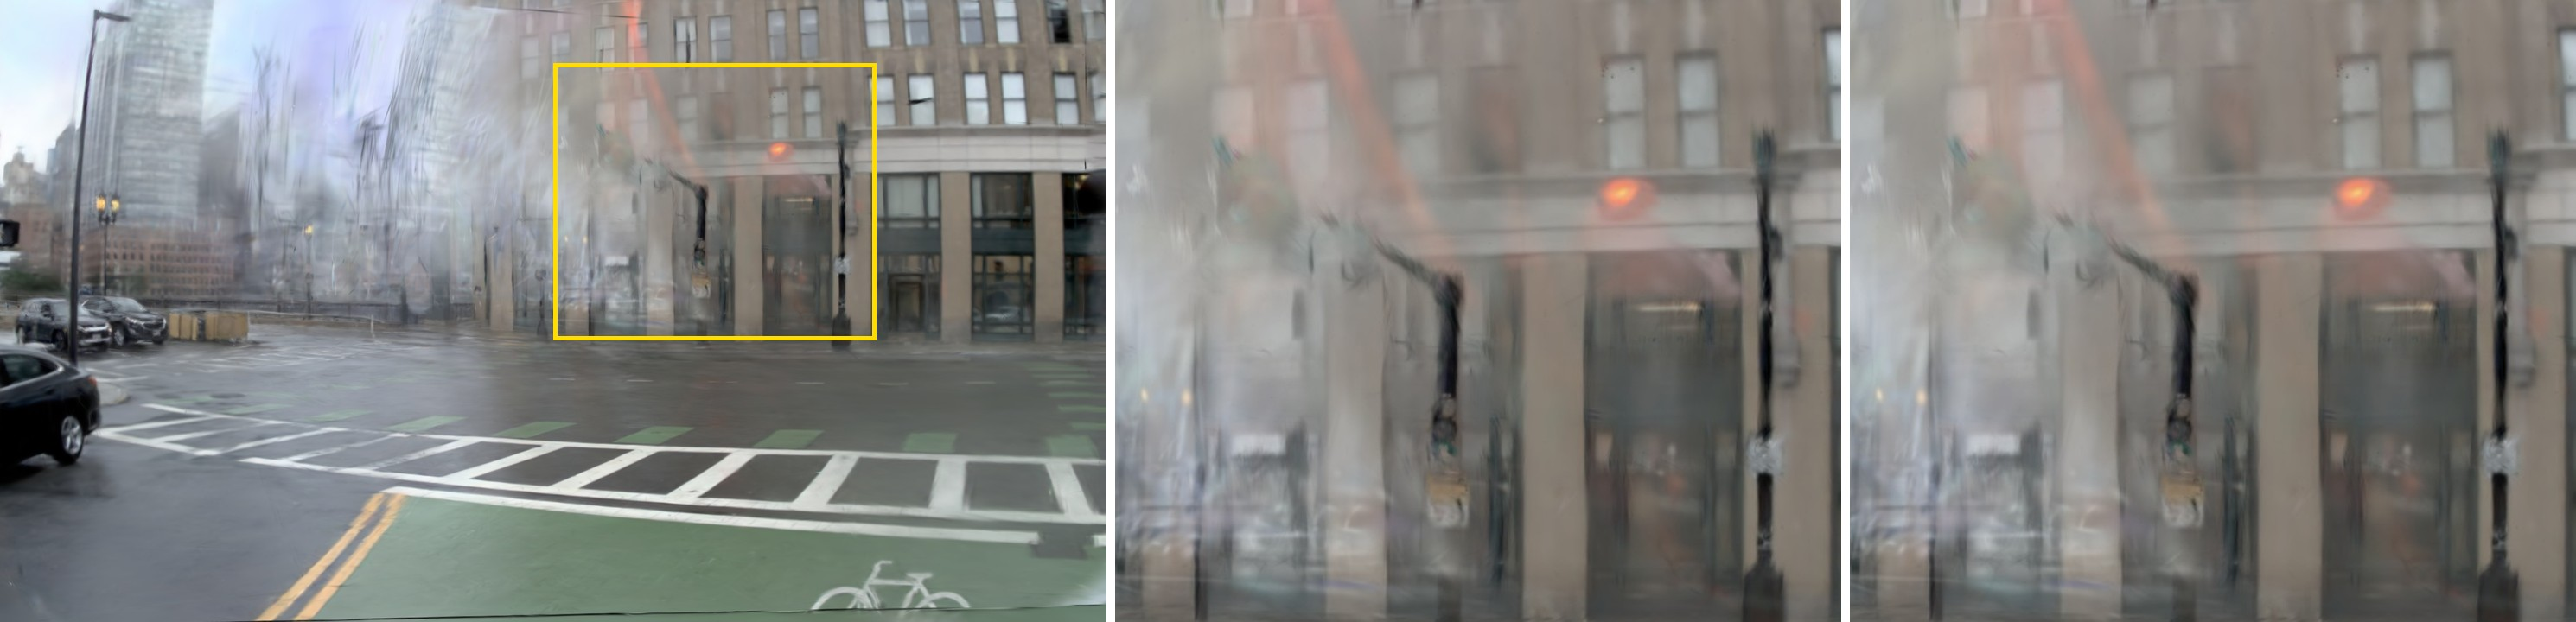
\includegraphics[width=\linewidth]{figures/rendered_signal_982b57b1.jpg}
\caption{Rendered front camera in a local stall rollout (public Boston scene \texttt{982b57b1}, rendered from the public track assets \cite{trackdata}, CC BY-NC-SA 4.0). Left: full frame 0.5 s after takeover; the box marks the crop. Middle and right: the crop at 0.5 s and at 5.0 s. The crops are unchanged (mean absolute pixel difference 0.4 of 255), although the logged human departed 2.0 s after takeover. The red glow that reads as a red signal lies on the facade, most likely a storefront light; the signal heads on the mast arm are ghosted.}\label{fig:signal}
\end{figure}
% Supplementary inventory, reviewed 2026-11-09; extended 2026-11-13 with the lf-012 entry and the November 10-13 items;
% extended 2026-11-18 with the lf-013 entry, the November 16 last-slot review and the post-deadline 2026-11-18 snapshot
% (leaderboard/2026-11-18/nuplan.json).
% Evidence comments are indexed in experiment-history-evidence-20261109.json and, for the 2026-11-13 additions,
% in experiment-history-evidence-20261113.json.
\section{Experiment history: August--November 2026}\label{app:history}
This inventory covers the completed experiment families and diagnostic work retained in our project records through November 17, 2026, the day of our final nuPlan entry. Repeated seeds, sweep points, checkpoint evaluations and infrastructure retries are grouped under their method. Proposed or prepared work is identified separately. Earlier comparisons used different checkpoints, scene subsets and evaluator revisions: their scores are historical observations, not a common benchmark or predictions of official PCS. All results below are local unless explicitly described as official. ``Perfect'' means score one, not a guarantee of correct or safe driving. Supporting records and hashes are indexed in the author's experiment records, available on request. Table~\ref{tab:entries} lists every official entry; the bullets that follow describe the work behind them.

\begin{table}[htbp]
\centering\footnotesize\setlength{\tabcolsep}{4pt}
\caption{All official nuPlan entries of Team Lucifer AI, with every value taken from the post-deadline November 18, 2026 leaderboard snapshot used for Table~\ref{tab:official} \cite{board}. PCS is refitted as entries are added, so these values differ from earlier dated records. In this snapshot \texttt{lf-013} has the 4th-highest PCS among the best entries of the 57 participating teams (286 entries in all). Dates are UTC submission dates unless footnoted. $^a$First submitted August 29 on the pre-reset 1,485-scene board (rank 6 of 19 teams, PCS 1590); after the move to the final scene set the board lists it with a September 16 date. $^b$Not named in our local records; in the October 21 snapshot its official mean matched the host's public \texttt{model\_0014} entry to four decimals (0.8479); the board has since recomputed both means (now 0.8519 and 0.8529).}\label{tab:entries}
\begin{tabular}{@{}lL{1.75cm}L{4.4cm}rrr@{}}
\toprule
Date & Entry & Policy & Mean $\uparrow$ & PCS [95\%] $\uparrow$ & km/inc. $\uparrow$ \\
\midrule
09-10 & \texttt{wajepa-s2} & WA-JEPA, two flow steps \cite{wajepa} & 0.7678 & 1149 [1085, 1213] & 0.626 \\
09-16$^a$ & \texttt{vavam-stock} & Stock VaVAM-B \cite{vavam} & 0.5580 & 863 [818, 908] & 0.106 \\
09-24 & untagged$^b$ & Public Py123d \texttt{model\_0014} & 0.8519 & 1501 [1428, 1575] & 0.228 \\
09-30 & \texttt{lf-007} & \texttt{model\_0014}, route bridge, scale 1.25 & 0.8820 & 1568 [1487, 1649] & 0.407 \\
10-12 & \texttt{B1} & \texttt{model\_0014}, fine-tuned planning head & 0.8767 & 1607 [1522, 1692] & 0.387 \\
10-21 & \texttt{lf-008} & C2 epoch 31 (full-model training), exact targets & 0.8931 & 1680 [1583, 1776] & 0.528 \\
10-30 & \lf{} & v0.2.0 waypoint seed 1, exact-arc route & 0.9454 & 2487 [2341, 2633] & 1.039 \\
11-06 & \texttt{lf-010} & SimScale step 1,024, Track A, lead rule & 0.9433 & 2367 [2218, 2515] & 0.929 \\
11-13 & \texttt{lf-012} & \lf{} weights, lead rule, 5$^\circ$ bend veto & 0.9462 & 2412 [2250, 2574] & 1.110 \\
11-17 & \texttt{lf-013} & \lf{} weights, 10$^\circ$ bend veto only & 0.9494 & 2502 [2317, 2687] & 1.364 \\
\bottomrule
\end{tabular}
\end{table}

\begingroup
\clubpenalty=10000
\widowpenalty=10000

\subsection{Early world/action-model baselines: VaVAM and WA-JEPA (August--September)}
\begin{itemize}\setlength{\itemsep}{3pt}\setlength{\parsep}{0pt}\setlength{\parskip}{0pt}\setlength{\topsep}{3pt}
% evidence: CURRENT-BEST.md | SETUP-NOTES.md
\item \textbf{Stock VaVAM-B and the initial submission.} Packaged the organizer's driver, established local evaluation and submitted the stock model on August 29 (rank 6 of 19 teams, PCS 1590 on the pre-reset board) \cite{vavam}. This provided the initial official reference before the leaderboard reset and subsequent WA-JEPA entry.
% evidence: CURRENT-BEST.md | README.md
\item \textbf{VaVAM $\mu$P correction and larger checkpoint.} Restored the checkpoint's expected parameterization/base shapes and compared VaVAM-B/$\mu$P \cite{vavam,mup} with stock and VaVAM-L/$\mu$P. Historical 400-scene means were 0.8813 versus 0.8493 for corrected-B versus stock; the larger L checkpoint regressed on its screen.
% evidence: CURRENT-BEST.md | SETUP-NOTES.md
\item \textbf{VaVAM inference variants.} Tested output gains, batched multi-plan sampling, route/discriminator-based selection and selection-weight sweeps. Gains could increase progress but introduced collisions; sample-selection improvements were small or inconsistent. Seed reproducibility and silent-fallback defects were corrected during these tests.
% evidence: CURRENT-BEST.md | README.md | SETUP-NOTES.md
\item \textbf{Simple driving controls.} Tested go-straight, route-following, braking-aware and constant-speed/route hybrids. The route follower reached a historical 400-scene mean of 0.8896, but the confirmed hybrid added collisions relative to corrected VaVAM. A better mean alone was insufficient.
% evidence: SETUP-NOTES.md | README.md
\item \textbf{WA-JEPA integration-step comparison.} Integrated WA-JEPA \cite{wajepa} and tested 2, 4 and 12 flow steps. S2/S4 reached 0.9247/0.9302 on the historical 400 scenes; S12 reached 0.9667 on a smaller 100-scene screen. S12 was not a matched 400-scene result. Early latency projections used stale official limits and were subsequently withdrawn.
% evidence: SETUP-NOTES.md
\item \textbf{WA-JEPA S2 official entry and diagnosis.} The September 10 record reports 1,000/1,000 valid rollouts, official mean 0.7748 and PCS 986, substantially below its local 0.9247. Route-command alternatives did not resolve the loss. Saved traces showed gradual lateral departure; this did not establish an out-of-distribution private dataset.
% evidence: README.md | py123d/MODEL.md
\item \textbf{GTRS-Dense and public Py123d comparisons.} Integrated the pretrained GTRS-Dense \cite{gtrs} adapter and evaluated 400 scenes: mean 0.8424, 61 zeros and no inference failures. The older Py123d \texttt{model\_0014} reference scored 0.8420 locally despite stronger official standing than WA-JEPA. This exposed the local benchmark's misleading model ordering.
\end{itemize}

\subsection{Cosmos3-Edge: frozen backbone and learned driving head (September)}
\begin{itemize}\setlength{\itemsep}{3pt}\setlength{\parsep}{0pt}\setlength{\parskip}{0pt}\setlength{\topsep}{3pt}
% evidence: cosmos3/COMPATIBILITY.md
\item \textbf{Full-checkpoint compatibility and native output.} Ran the full Cosmos3-Edge \cite{cosmos3edge,cosmos} generator/VAE with its camera-action adapter on one AlpaSim scene: 10/10 model calls, no fallback, approximately 2.48 s per call and 10.1 GiB sampled process VRAM. The rollout nevertheless exited the corridor, scored zero and reached only 29.6\% relative progress.
% evidence: cosmos3/LOCAL-HEAD10-RESULT.md | cosmos3/ABLATION-RESULT.md
\item \textbf{Ten-example head-training smoke test.} Trained an approximately 815,000-parameter waypoint head on frozen Cosmos features, verifying optimization, checkpoint reload and unchanged backbone weights. A vehicle-state convention issue was found and corrected. This was a pipeline test, not evidence of driving improvement or Cosmos-backbone fine-tuning.
% evidence: cosmos3/ABLATION-RESULT.md
\item \textbf{Visual-feature ablation.} Compared the frozen-Cosmos head with a state/route-only head on a tiny recording-separated pilot. On nine held-out examples, ADE was 2.414 m versus 1.977 m: adding these Cosmos features did not establish an advantage.
% evidence: cosmos3/STEPWISE-RUN-20260921.md
\item \textbf{Larger four-city real-camera pilot.} Expanded to 26 independent recordings: 19 training and seven validation, with 2,666/631 windows and 7,188 unique images. Both heads trained for 840 updates with Cosmos frozen. Visual-head ADE/FDE was 1.192/3.009 m versus 1.150/3.076 m for state/route-only: mixed metrics, no visual ADE advantage in any city. The learned head was not advanced to a 400-scene closed-loop comparison.
% evidence: cosmos3/STEPWISE-RUN-20260921.md | cosmos3/ABLATION-RESULT.md
\item \textbf{Camera and training-data readiness.} Audited real/simulated observations, temporal history, timestamp alignment, ego-state construction and whole-recording separation before feature caching. These checks made the pilot executable; neither they nor the small fits demonstrated Odyssey-style \cite{odyssey} transfer or a leaderboard-ready world-model policy.
\end{itemize}

\subsection{Older Py123d checkpoint: controller, trajectory and route changes (September--October)}
\begin{itemize}\setlength{\itemsep}{3pt}\setlength{\parsep}{0pt}\setlength{\parskip}{0pt}\setlength{\topsep}{3pt}
% evidence: README.md
\item \textbf{MPC and stabilization sweeps.} Swept longitudinal/lateral tracking, acceleration and related controller costs, trajectory blending and output conventions on small development panels. Large development improvements shrank on the 141-scene comparison; the selected controller configuration improved the historical mean only from approximately 0.8523 to 0.8549.
% evidence: README.md
\item \textbf{Optuna search.} Ran, with Optuna \cite{optuna}, 36 completed trials of a planned 50-trial controller/stabilization search, followed by checks of trials 26 and 21. Trial 26 improved the 141-scene historical mean by about 0.0044, without reducing corridor failures. The development optimum was not a reliable estimate of general improvement.
% evidence: openai_golf/RESULTS-2026-09-27.md
\item \textbf{Prediction-versus-execution audit and predicted yaw.} Compared route inputs, planned paths and executed trajectories on corridor failures; tracking errors were much smaller than planned-path deviations. In fresh paired 141-scene tests, predicted yaw improved mean score by 0.0198 and corridor exits fell from eight to five; adding controller tuning gave only a small further gain.
% evidence: openai_golf/RESULTS-ROUTE-BRIDGE-2026-09-27.md | openai_golf/RESULTS-ROUTE-VALIDATION-2026-09-27.md | openai_golf/submission-20261021-c2-e31-exact/README.md
\item \textbf{Route bridging and early driver entry.} Built a smooth bridge over the missing near-route segment, tested heading/route conditioning and trajectory scale, and packaged the route-bridge/scale-1.25 variant as \texttt{lf-007}. These older-checkpoint modifications preceded the later exact-arc correction used by \lf{}.
% evidence: openai_golf/RESULTS-2026-10-07-SCALE150-CHALLENGER.md | openai_golf/RESULTS-2026-10-08-TARGET40-CHALLENGER.md | openai_golf/RESULTS-2026-10-08-TARGET50-CHALLENGER.md | openai_golf/RESULTS-2026-10-09-SMALL-TWEAK-BATCH.md
\item \textbf{Follow-up route and controller ablations.} Tested scale 1.5, 40/50 m targets, bridge tangents, direction fitting, controller gains and stabilization. Small-panel successes did not yield a convincing broad upgrade; some settings introduced failures. Fresh baseline reruns also showed why historical references could misattribute a regression.
% evidence: openai_golf/stage1-2026-10-14/README.md | openai_golf/CURRENT-BEST-2026-10-21.md
\item \textbf{Early off-road veto and progress warp.} Tried predicted-road-based lateral ramp candidates, straight-plan time warping and their combination on the older checkpoint. Small-panel rescues justified expansion, but the full 1,470-scene warp/bundle check introduced new zeros. These rules were excluded from the C2 submission.
\end{itemize}

\subsection{Real-data Py123d adaptation and larger training runs (October)}
\begin{itemize}\setlength{\itemsep}{3pt}\setlength{\parsep}{0pt}\setlength{\parskip}{0pt}\setlength{\topsep}{3pt}
% evidence: openai_golf/RESULTS-2026-10-09-FINETUNE-RUNS.md | openai_golf/RESULTS-2026-10-09-PILOT-CONFIRMATION.md
\item \textbf{Frozen-feature planning-head fine-tuning.} Adapted roughly 9.6M planning parameters of \texttt{model\_0014} using independent nuPlan/OpenScene recordings, with representative, departure, stop and turn sampling. Tested learning rates, epochs and braking/false-go guards. The selected early pilot improved local closed-loop results, motivating larger trials.
% evidence: openai_golf/departure-balance-2026-10-10/RESULTS.md | openai_golf/departure-balance-2026-10-10/panel-result.json | openai_golf/RESULTS-2026-10-10-OFFROAD-BEND-EXPERIMENT.md
\item \textbf{Departure and tight-bend reweighting.} Trained immediate-departure versus unchanged-sampler heads and a low-clearance bend challenger. Departure reweighting reduced mean score by 0.0030 on 197 scenes. The bend challenger rescued one additional failure in its 139-scene check but worsened many successful tight-margin controls and was not advanced.
% evidence: openai_golf/RESULTS-2026-10-12-B-ARMS.md | openai_golf/submission-20261012-b1/README.md
\item \textbf{Larger head-training pools and B-series variants.} Expanded recordings, changed city/Singapore sampling and increased training duration. B1 passed its local comparison and was submitted; its official mean was lower than the preceding route-bridge entry. More local training and a positive screen did not guarantee transfer.
% evidence: openai_golf/training-2026-10-16/README.md
\item \textbf{Full-model C0 and C1 training.} Moved beyond frozen-head adaptation: C0 trained on approximately 184,000 cached examples; C1 expanded to approximately 372,000 candidate anchors. C1 completed ten epochs before a reboot interrupted the longer plan. Closed-loop gains improved even as open-loop validation error worsened, demonstrating that these measurements were not interchangeable.
% evidence: openai_golf/training-2026-10-16/README.md | openai_golf/submission-20261021-c2-e31-exact/README.md
\item \textbf{Two-PC data expansion and C2.} Combined caches from two machines, with approximately 622,000 indexed training anchors and city-balanced sampling; cache-valid counts were slightly lower. Trained and compared multiple C2 checkpoints. Epoch 31 plus exact route targeting became \texttt{lf-008}, with an official mean improvement over \texttt{lf-007} in the same October 21 snapshot. Larger-data training did help this earlier base policy.
% evidence: openai_golf/PLAN-2026-10-18-NAVTEST-TRAINING.md | openai_golf/CURRENT-BEST-2026-10-21.md
\item \textbf{K/M/N continuation ablations.} Tested continued training (K), live road/walkway/centreline supervision (M), and additional, explicitly separated public-navtest training recordings (N). None improved on C2 epoch 31 on the clean comparison; N regressed by 0.0143 over all 659 scenes. Recordings used by N cannot be counted as untouched evaluation for that arm.
% evidence: openai_golf/boundary-probe-2026-10-10/RESULTS.md | openai_golf/RESULTS-2026-10-10-OFFROAD-BEND-EXPERIMENT.md
\item \textbf{Road-boundary and auxiliary-perception diagnostics.} Audited human-path clearance, predicted road/object heads, map labels and differentiable boundary-loss feasibility. Some human trajectories themselves violated the evaluator's mapped boundary. These probes did not establish a deployable road-safety filter or justify shifting every prediction laterally.
% evidence: openai_golf/boundary-probe-2026-10-10/RESULTS.md
\item \textbf{Boundary-loss head training.} Trained a weak boundary-loss probe, rejected on braking guards, then a stronger boundary-plus-braking variant. The latter passed offline guards but tied its pilot reference on 196 scenes: 63 zeros each, with one off-road rescue and one new off-road failure. It was not promoted.
\end{itemize}

\subsection{Released v0.2.0 checkpoints and the lf-009 interface (late October)}
\begin{itemize}\setlength{\itemsep}{3pt}\setlength{\parsep}{0pt}\setlength{\parskip}{0pt}\setlength{\topsep}{3pt}
% evidence: openai_golf/STATE-2026-10-30-FINDINGS-AND-NOVEMBER-PLAN.md | openai_golf/PLAN-2026-10-18-NAVTEST-TRAINING.md
\item \textbf{New pretrained waypoint/joint checkpoints.} Replaced the older development base with the released approximately 68M waypoint-flow policy \cite{weights}, a latent TransFuser \cite{transfuser} variant, and compared seeds and joint action/waypoint variants. The host's new checkpoints were externally trained releases, not models trained from scratch by our team.
% evidence: openai_golf/STATE-2026-10-30-FINDINGS-AND-NOVEMBER-PLAN.md | openai_golf/PLAN-2026-10-18-NAVTEST-TRAINING.md
\item \textbf{Route memory, extrapolation and ensembles.} Evaluated route memory, extrapolation, a three-seed prediction ensemble, whole-model weight averaging \cite{soups} and backbone-only averaging. None supplied a robust replacement for the selected single checkpoint; extrapolation and some combinations caused new failures. Route memory's benefit largely disappeared after exact target placement.
% evidence: openai_golf/overnight-20261030/RESULTS.md | openai_golf/overnight-20261030/OUTPUT-ABLATION.md
\item \textbf{Joint64 output-mode ablations.} Compared native waypoints, integrated actions and speed-dependent action/waypoint hybrids. Changes could trade off off-road failures against collisions or stalls; larger checks did not establish an upgrade over the waypoint reference.
% evidence: openai_golf/STATE-2026-10-30-FINDINGS-AND-NOVEMBER-PLAN.md | technical_report/evidence-20261108.json
\item \textbf{Exact-arc targets and keeping the served route whole.} Corrected route-target placement and avoided truncating the served polyline. Exact targeting improved mean score by 0.0054 and reduced zeros from 62 to 52 on the matched 1,473-scene comparison. The unchanged seed-1 checkpoint with these interface fixes became \lf{}, the base of all our later entries.
% evidence: openai_golf/PLAN-2026-10-18-NAVTEST-TRAINING.md | openai_golf/headcheck-v020-2026-10-29/README.md
\item \textbf{Checkpoint/interface parity checks.} Checked camera preprocessing, historical frames, speed inputs, route encoding, output coordinates and auxiliary head accuracy. Camera redistortion did not improve the diagnostic result. Successful inference was not treated as proof that input semantics or near-road geometry were correct.
\end{itemize}

\subsection{SimScale recovery adaptation: original pilots, corrections and scaling (October--November)}
\begin{itemize}\setlength{\itemsep}{3pt}\setlength{\parsep}{0pt}\setlength{\parskip}{0pt}\setlength{\topsep}{3pt}
% evidence: openai_golf/simscale-screen-2026-11-01/README.md
\item \textbf{Original recovery pilot and long1 run.} Mixed SimScale \cite{simscale} synthetic recovery and real nuPlan data equally; screened step 500 of the 3,000-step run. On 231 hard scenes it removed a net 21 incidents and 17 deep stalls, but introduced nine incidents on 378 easy scenes. The optimistic weighted 331-scene forecast did not survive the larger easy-scene check.
% evidence: openai_golf/simscale-screen-2026-11-01/README.md | openai_golf/path1-inference-audit-2026-11-02/CROSS-VALIDATION.md
\item \textbf{Gentle1 and state-based model switching.} Lowered learning rate and synthetic share, trained 400 steps and tested both hard/easy groups: only four net hard incidents removed, with five new easy incidents. Separately, retrospective route-heading/speed selectors between base and recovery models failed recording-level cross-validation; their apparent training-set gain was not robust.
% evidence: openai_golf/simscale-screen-2026-11-01/README.md
\item \textbf{Driver-side bias correction of step 500.} A constant lateral offset compounded under replanning and was stopped. Speed-dependent lateral/heading correction removed the measured average bias but still caused seven easy-scene incidents while retaining 17 net hard-scene rescues. The prebuilt 50/50 base/step-500 blend was not evaluated; this is separate from the later tested 30\% interpolation.
% evidence: openai_golf/PLAN-2026-11-02-TWO-PATHS.md | openai_golf/path1-inference-audit-2026-11-02/CROSS-VALIDATION.md
\item \textbf{Conversion and label repairs.} Diagnosed synthetic-tail contamination of real labels, inappropriate temporal re-gridding, source-window split leakage, batch recycling, missing normalization buffers and route/timestamp errors. Rebuilt corrected corpora, masked supervision to the observed four seconds and introduced source-recording protection. Earlier failed runs were not reinterpreted as clean tests of the corrected recipe.
% evidence: openai_golf/PLAN-2026-11-02-TWO-PATHS.md
\item \textbf{Curated 5,000-anchor decoder pilot.} Filtered perturbations, speed and label plausibility, reduced synthetic share and anchored ordinary driving to \lf{}. Recovery accuracy improved, but correction was asymmetric and rendered predictions leaned right. This pilot was stopped before a closed-loop candidate test.
% evidence: openai_golf/simscale-clean-pilot-2026-11-03/README.md | openai_golf/simscale-training-2026-11-03/RESULTS.md | openai_golf/simscale-preservation-queue-2026-11-03/RESULTS.md
\item \textbf{Independent clean pilot and preservation A/B tests.} Built a 256-example, 97-recording recovery pilot and verified training with a frozen backbone. A 64-step CPU fit improved held-out lateral error by only about 5 mm. Subsequent A/B fits tested rendered-preservation examples: preservation improved, but recovery gains remained negligible.
% evidence: openai_golf/simscale-label-control-2026-11-03/RESULTS.md | openai_golf/two-track-queue-2026-11-03/RESULTS.md
\item \textbf{Loss-path controls and longer small-pool fits.} Tested label/gradient controls, then extended the A/B arms to 1,024 steps. Recovery gains remained only approximately 2.6--3.1 cm while real-image deviation rose above 0.12 m; both continuations stopped on guards. Duration alone did not fix the trade-off.
% evidence: openai_golf/simscale-data-v3-2026-11-03/README.md | openai_golf/simscale-v3-lean-2026-11-04/RESULTS.md | openai_golf/label-semantics-check-2026-11-04/README.md
\item \textbf{V3 residual-balanced pairs and lean test.} Paired opposite residuals within city/turn/speed groups and included rendered controls. The 256-step test stopped on a recovery-set shift guard; ordinary preservation checks passed, so this alone did not prove global lean. Full-horizon audits showed initially outward-moving recovery labels and unequal directional gains despite endpoint balancing.
% evidence: openai_golf/route-recache-2026-11-04/PILOT-RESULTS.md | openai_golf/simscale-final-reserved-2026-11-04/README.md
\item \textbf{Corrected route recache and reserved-recording pilot.} Rebuilt teacher features after correcting route construction/alignment and retested decoder adaptation. The corrected step-512 model showed recovery improvement under the preservation checks, justifying selection from the larger corrected corpus.
% evidence: technical_report/evidence-20261108.json | openai_golf/simscale-fullpool-2026-11-04/PLAN.md
\item \textbf{Expanded recovery pool, steps 256/512/768/1,024.} Selected 3,412 recovery anchors with city-balanced paired sampling, 2,272 rendered controls and 512 real controls. Step 512 plus both inference rules reached mean 0.9272 and 40 incidents; step 1,024 plus both rules reached 0.9303 and 38 incidents, versus 0.9132/52 for \lf{}, on 1,472 local scenes.
% evidence: technical_report/evidence-20261108.json
\item \textbf{Official SimScale submission, lf-010.} Submitted the corrected step-1,024 model together with the lead rule and Track A. In the same November 6 snapshot, mean score was 0.9433 versus \lf{}'s 0.9454, despite the local gain. This bundled comparison cannot identify whether weights, selectors or their interaction caused the negative transfer.
% evidence: openai_golf/simscale-recovery-3412-2026-11-05/outputs/RESULTS.md | openai_golf/simscale-recovery-3412-2026-11-05/outputs/REPORT.md
\item \textbf{Longer 3,412-step city-balanced run.} Evaluated checkpoints at 1,536/2,048/2,560/3,072/3,412 steps; most passed the reserved open-loop gates, while step 2,560 failed. The run visited 2,736 distinct recovery anchors (80.2\% of the pool), not every anchor once. In closed loop with both inference rules, steps 2,048 and 3,412 raised the weighted 609-scene score by 0.0195 and 0.0198 over \lf{} (35 and 32 at-fault incidents), but step 2,048 repeatedly went off road on an easy 863-panel scene that every other model passed, and step 3,412 added four new zeros on easy scenes. Neither was submitted: longer training fixed more hard scenes but broke easy ones.
% evidence: openai_golf/wise-ft-2026-11-07/README.md
\item \textbf{Same-initialization weight interpolation.} Following WiSE-FT \cite{wiseft}, tested 30\% of the corrected fine-tune delta with unchanged hooks. At 556 development scenes, compared with hooks alone, it removed no additional incident and lost three perfect scenes. The blend was stopped; reducing weight displacement did not preserve the desired gains in that test.
\end{itemize}

\subsection{Inference-only changes around lf-009 (November)}
\begin{itemize}\setlength{\itemsep}{3pt}\setlength{\parsep}{0pt}\setlength{\parskip}{0pt}\setlength{\topsep}{3pt}
% evidence: openai_golf/inference-paper-2026-11-02/README.md | openai_golf/inference-paper-2026-11-02/paired-repair.log | openai_golf/inference-paper-2026-11-02/paired-smooth.log
\item \textbf{Paper-inspired trajectory refinement.} Implemented bounded acceleration/curvature projection and smoothing: neither changed any score on the paired 32-scene test. Predicted-box collision margins, braking retiming and progress proposals were also exercised in shadow mode. These were limited adaptations, not reproductions of complete learned safety-filter methods or proven safety guarantees.
% evidence: openai_golf/inference-route6080-609-2026-11-02/README.md | openai_golf/inference-route6080-609-2026-11-02/report.json
\item \textbf{Dropping the 40 m route target.} A native 60/80 m-only mask rescued one collision on a 32-scene diagnostic panel. The fresh paired 609-scene study instead reduced the weighted mean by 0.0058 and increased zeros from 52 to 55. Rejected; this ablation is distinct from exact-arc target placement.
% evidence: technical_report/evidence-20261108.json | openai_golf/lead-guards-2026-11-07/RESULTS.md
\item \textbf{Lead-departure rule and targeted guards.} Advanced slowly moving plans when predicted lead motion and existing intent supported departure. Across the corrected 1,472-scene comparison, lead-only improved mean by 0.00566, improved 32 scores and worsened none. Motion/path-support vetoes reduced gains on targeted checks; unchanged scores during four human-wait intervals did not prove safe waiting behavior.
% evidence: technical_report/evidence-20261108.json
\item \textbf{Track A and combined rules.} Sampled 16 policy plans and selected using predicted road/object checks when the default failed. Track A showed a small 609-scene gain with uncertainty spanning zero. The actual combined lead-plus-selector run improved locally; it remained necessary to test the combination, rather than assume separate gains add.
% evidence: openai_golf/speed-test-2026-11-04/README.md
\item \textbf{Uniform speed retiming.} Tested a 1.05 speed multiplier on the SimScale-512/combined-rule candidate. Progress increased on many scenes, but zeros rose from 41 to 50 on 609 scenes, including new easy-scene failures. Rejected; the proposed 1.10 arm was not run.
% evidence: openai_golf/centre-probe-2026-11-06/README.md
\item \textbf{Predicted-centreline warning probe.} Logged 62 development scenes without changing driving. A candidate-switching rule could warn early for eight of 22 incident scenes, but also activated in eight of 40 clean scenes. No larger intervention run was justified by this diagnostic.
% evidence: openai_golf/bendveto-2026-11-11/README.md | openai_golf/bendveto-2026-11-11/closedloop-result.json | openai_golf/bendveto-2026-11-11/why-limited.json
\item \textbf{Bend veto.} Shifted the nominal plan laterally by 0.5 or 1.0 m when it bent by at least 10$^\circ$ and the policy's own predicted road map gave probability below 0.5 under the planned footprint, provided the shifted plan was clearly better supported and touched no predicted vehicle. On the 1,472 scenes it removed 10 of 52 incident scenes, added none and lost no score-one scene (mean 0.9132 to 0.9200). Its reach is limited: it acted in 12 of the 44 off-road failures; 16 others show no low-road signal in the predicted map and 11 have bends below 10$^\circ$.
% evidence: openai_golf/leadveto-2026-11-11/README.md | openai_golf/leadveto-2026-11-11/closedloop-result.json
\item \textbf{Lead rule plus bend veto.} Combined both rules in one image, without Track A sampling. They never acted in the same scene: the lead rule in 58 scenes, the veto in 47. The mean rose to 0.9257 and incident scenes fell from 52 to 42, with 18 score-one scenes gained and none lost.
% evidence: openai_golf/PLAN-2026-11-12-QUICK-WINS.md | openai_golf/candidate-b-2026-11-12/README.md | openai_golf/candidate-b-2026-11-12/step2.json | openai_golf/candidate-b-2026-11-12/step4.json
\item \textbf{Pre-registered extensions: lead follow-through and a 5$^\circ$ bend limit.} Pass rules were fixed before any run, on development and confirmation halves of the 44 public recordings; both halves had appeared in earlier full runs, so this guarded against tuning rather than providing an independent test. A follow-through extension of the lead rule harmed no scene but gained 0.69 scene-score units on 23 development scenes against a required 0.8, and was dropped without retuning. Lowering the bend limit to 5$^\circ$ passed: on the full 1,472 scenes it differs from the 10$^\circ$ version in exactly four scenes, three off-road failures becoming score one and one scene falling from 0.999 to 0.931. Result: mean 0.9277, 39 incident scenes, 21 score-one scenes gained and none lost.
% evidence: openai_golf/submission-20261112-bend5/README.md | openai_golf/LEADERBOARD-NUPLAN-2026-11-13c.json
\item \textbf{Third entry, \texttt{lf-012}.} Submitted the rule-only variant (\lf{} weights, lead rule, 5$^\circ$ bend veto) on November 13 after a 32/32 warm-up. Its official mean (0.9462) and incident distance (1.110 km) exceed \lf{}'s, but its PCS was 2261 against 2302 in the November 13 snapshot (2412 against 2487 in the final one), with overlapping intervals. Local selection on score-one retention and incident counts, adopted after \texttt{lf-010}, therefore also failed to predict the official PCS ordering.
% evidence: openai_golf/controller-gains-2026-11-13/README.md | openai_golf/controller-gains-2026-11-13/track-gap.json
\item \textbf{Controller-tracking audit.} Compared planned with driven motion over 12,078 plans from the 1,342 scenes of that run in which no rule acted. The car follows the plan closely (driven-to-requested distance 1.02 at the median), and stalls coincide with plans that request almost no motion. No controller-gain variant was therefore run or submitted.
% evidence: openai_golf/last-slot-2026-11-16/README.md | openai_golf/last-slot-2026-11-16/rule_footprint.py | openai_golf/last-slot-2026-11-16/veto_bend.py
\item \textbf{Last-slot review: which rule cost \texttt{lf-012} its PCS.} Re-read the saved full local runs of \lf{}, veto-only, lead-only, both rules at 10$^\circ$ and \texttt{lf-012}. Both rules were clean locally: the 10$^\circ$ veto acted in 47 scenes and every one of the 32 that were perfect under \lf{} stayed perfect; the lead rule acted in 58 and only ever raised progress. Local data therefore could not assign \texttt{lf-012}'s official loss to either rule. Officially its distance to the human path rose 3.0\% against 1.5\% locally, so its rules acted more on the hidden recordings. All 10 local veto fixes lie on bends of 12.8--27.8$^\circ$, so a sharper gate would not have helped.
% evidence: openai_golf/submission-20261117-vetoonly/README.md | openai_golf/submission-20261117-vetoonly/official-submit.json | leaderboard/2026-11-18/nuplan.json
\item \textbf{Final entry, \texttt{lf-013}.} Submitted the veto alone at 10$^\circ$ (\texttt{lf-012}'s image with the lead rule off), the smallest change with a clean full local run, on November 17; because of the deadline it was sent while its warm-up was still queued, and the warm-up (32/32) succeeded afterwards. It is the only post-\lf{} entry whose official mean (0.9494), incident distance (1.364 km) and PCS (2502 against 2487) all rose, with overlapping PCS intervals. Duplicating \lf{} to redraw its interval, a 5$^\circ$ veto alone and any untested gate were rejected.
\end{itemize}

\subsection{PDM labels and learned candidate scorers (November)}
\begin{itemize}\setlength{\itemsep}{3pt}\setlength{\parsep}{0pt}\setlength{\parskip}{0pt}\setlength{\topsep}{3pt}
% evidence: openai_golf/centring-2026-11-06/README.md
\item \textbf{Real-data centred-label training.} Cached 12,202 real-image anchors, including 1,857 eligible label edits, and ran nine centring/preservation variants with different learning rates, balancing and loss weights. Stronger fitting also increased global lean; no tested setting established conditional centring without preservation damage. No closed-loop candidate was advanced.
% evidence: openai_golf/pdm-conversion-2026-11-05/README.md | openai_golf/pdm-expansion-2026-11-06/README.md
\item \textbf{PDM conversion, parity and expansion.} Converted 4,979 of the initial 5,000 SimScale clips \cite{simscale}, whose labels come from a PDM-style rule-based planner \cite{pdm}; 21 lacked required sources. Audited raw/converted poses, routes, images, timing, labels and trainer compatibility; investigated teacher-cache numerical parity before expanding selection. PDM trajectories were not assumed to be human-line recovery labels and required explicit slowdown checks.
% evidence: openai_golf/pdm-lateral-audit-2026-11-06/README.md | openai_golf/pdm-lateral-pilot-2026-11-06/outputs/RESULTS.md
\item \textbf{PDM lateral-only training.} After full-trajectory pairing proved restrictive, trained a small speed-matched lateral adaptation from 33 pairs. Step 256 improved lateral error by 3.3 cm but failed preservation checks; it was not extended to step 512 or closed-loop evaluation. This does not rule out all PDM uses.
% evidence: openai_golf/scorer-feasibility-2026-11-06/README.md | openai_golf/scorer-pilot-2026-11-06/README.md
\item \textbf{Frozen-driver learned scorer pilot.} Trained a small candidate-ranking head, a reduced form of learned trajectory scoring \cite{hydramdp,gtrs}, while keeping \lf{}'s weights unchanged. Offline ground-truth road geometry graded candidates but was not an inference input. Conservative guards left no demonstrated held-out rescues; simply taking the highest scorer output could introduce regressions.
% evidence: openai_golf/scorer-recovery-2026-11-06/README.md
\item \textbf{Recovery-state scorer feasibility and sampler repair.} Expanded recovery examples, audited motion/progress constraints and corrected the cached sampling stream to match Track A. Too few useful alternatives survived the fixed guards, so this corpus did not advance to another scorer fit. A selector cannot recover a path absent from its candidate set.
% evidence: openai_golf/scorer-boundary-mining-2026-11-06/README.md
\item \textbf{Boundary-mined scorer.} Mined road-exit states from independent training data and fitted an approximately 241,000-parameter residual scorer. It achieved three development rescues versus four for the existing heuristic, and zero confirmation rescues, matching the confirmation oracle ceiling. No simulator or official improvement was established.
\end{itemize}

\subsection{RoaD-inspired on-policy and shadow-label adaptation (November 7--9)}
\begin{itemize}\setlength{\itemsep}{3pt}\setlength{\parsep}{0pt}\setlength{\parskip}{0pt}\setlength{\topsep}{3pt}
% evidence: openai_golf/road-pilot-2026-11-07/RESULTS.md | openai_golf/road-long-capture-2026-11-07/RESULTS.md | technical_report/evidence-20261108.json
\item \textbf{Guided collection and decoder distillation.} Following RoaD \cite{road}, collected policy rollouts with 64 sampled plans, logged-human guidance and recovery blending; trained only the flow denoiser with real/rendered preservation. Expanded collection, repaired startup-history reconstruction and compared repeated collection rounds. The 48-scene paired test in the main report showed no convincing general learned-policy gain.
% evidence: technical_report/evidence-20261108.json | openai_golf/road-unguided-labels-2026-11-08/README.md
\item \textbf{Earlier intervention and rounds 1--3.} An earlier-intervention privileged teacher rescued three off-road failures on 24 scenes. Learned round-2 step 768 improved its training panel and rescued failures on other recordings, but lost one of 24 previously perfect controls on the reused 55-scene panel. Round 3 matched round 2 (five zeros on the 24 training scenes): guided rounds saturated because their labels sat on the human line (median 0.005--0.11 m), not at the 0.3--1.1 m offsets from which \lf{} actually fails.
% evidence: openai_golf/road-unguided-labels-2026-11-08/README.md
\item \textbf{Unguided-state shadow labels, U and U+.} Motivated by DAgger \cite{dagger} and the rollout-guided preventive supervision of RoG-DAgger \cite{rogdagger}, let \lf{} execute its nominal plan while recording feasible teacher alternatives at pre-departure states. Only 17 labels from seven scenes survived: at 28 of 78 pre-departure states, none of \lf{}'s 64 samples stayed on the road for 2 s, so once about 0.5 m off its line the policy's own samples contained no recovery to select. Trained shadow-only U and mixed U+; U-1024 reduced training-panel zeros from seven to three and initially preserved all 24 perfect controls on the 55-scene panel. U was exploratory because its label count missed the primary-arm minimum.
% evidence: openai_golf/road-unguided-labels-2026-11-08/README.md
\item \textbf{Mixture and preservation diagnostics.} U+ underperformed U, but used about 12.5 times fewer shadow-label draws, so this did not isolate harm from guided labels. U-1024 already failed open-loop rendered-deviation/lean checks. Its small-panel success was therefore treated as provisional, not evidence that preservation guards were unnecessary.
% evidence: openai_golf/road-unguided-labels-2026-11-08/README.md
\item \textbf{Larger U-1024 development check: rejected.} Stopped at 417 of 814 planned scenes: incidents stayed at 11, with two removed and two new off-road zeros on previously perfect scenes. Partial-scene scores improved and the weighted mean rose by 0.0075, but the preservation/incident gates failed. No protected-final evaluation or submission followed. Constructed preventive-label expansion remained a proposal at this review cutoff.
\end{itemize}

\subsection{Evaluation, data and diagnostic work supporting these experiments}
\begin{itemize}\setlength{\itemsep}{3pt}\setlength{\parsep}{0pt}\setlength{\parskip}{0pt}\setlength{\topsep}{3pt}
% evidence: README.md | openai_golf/RESULTS-2026-10-09-FULL1485-INCUMBENT.md | technical_report/evidence-20261108.json
\item \textbf{Broader public coverage and paired comparisons.} Expanded beyond the initial 400 scenes to the 1,485-scene public manifest, with usable matched denominators explicitly recorded per run. Added city/source-recording summaries, hard/easy controls, recording-bootstrap uncertainty and protected splits. Later 1,470/1,472/1,473-scene results are not silently treated as identical datasets.
% evidence: openai_golf/PCS-SENSITIVITY-2026-11-06.md | technical_report/evidence-20261108.json
\item \textbf{Metric and baseline audits.} Recomputed official scene-score components, investigated corridor scoring, corrected non-reproducing historical baselines and fitted local Drive-IRT \cite{driveirt} with score-one transitions. Local PCS improved some model orderings but still missed the \texttt{lf-010} reversal. Private-score sensitivity edits were diagnostics, not a universal PCS exchange rate.
% evidence: openai_golf/offroad-analysis-2026-11-01/README.md | openai_golf/road-unguided-labels-2026-11-08/README.md
\item \textbf{Failure casebooks and state-distribution analysis.} Separated corner cutting, straight-road drift, mapped-edge/human-path conflicts, collisions and stalls; compared supplied routes, planned paths and execution. Later shadow captures demonstrated that guided demonstrations often missed the actual pre-departure states reached by the unguided policy.
% evidence: openai_golf/departure-audit-2026-11-02/README.md | technical_report/figures/rendered_signal_982b57b1.jpg
\item \textbf{Departure cues and rendered traffic lights.} Audited 24 departure and 12 wait events in nuPlan frames: a visible reason explained 11 of 12 waits and about 15 of 24 departures, and no red-to-green change fell inside any departure window. In six stall rollouts the rendered lights stayed unchanged for 5 s while the logged human departed (Appendix~B, Figure~\ref{fig:signal}). We therefore treat signal stalls as outside the reach of our rules and built no rule that departs at a rendered red light.
% evidence: openai_golf/pdm-conversion-2026-11-05/README.md | openai_golf/simscale-fullpool-2026-11-04/PLAN.md | openai_golf/training-2026-10-16/README.md
\item \textbf{Data integrity and scaling infrastructure.} Built source-log exclusions, whole-recording splits, temporal/image/calibration checks, frozen-teacher caches, portable second-PC handoffs and checkpoint retention. Added SSD staging and resumable queues. Downloaded, converted, cached, selected and actually sampled counts were tracked separately; not all available data was trained on.
\end{itemize}

\subsection{Reviewed or prepared alternatives, not completed driving improvements}
\begin{itemize}\setlength{\itemsep}{3pt}\setlength{\parsep}{0pt}\setlength{\parskip}{0pt}\setlength{\topsep}{3pt}
% evidence: openai_golf/DATASET-SURVEY-2026-10-30.md | openai_golf/PLAN-2026-11-03-TWO-TRACKS.md
\item \textbf{Other data sources.} Probed or audited LEAD \cite{lead} perturbed-view data, nuReasoning \cite{nureasoning} and nuScenes \cite{nuscenes}, and surveyed CASCADE \cite{cascade}, PhysicalAI-AV \cite{nvidiadata}, DriveCoT \cite{drivecot}, WorldEngine \cite{worldengine} and others. These are not reported as trained challenge models. Departure/wait mining and additional downloads likewise do not constitute a completed fine-tune by themselves.
% evidence: alternative_models/alt_model.md | openai_golf/PLAN-2026-10-18-NAVTEST-TRAINING.md | cosmos3/STEPWISE-RUN-20260921.md
\item \textbf{Uncompleted model/architecture proposals.} Reviewed alternatives including HDP \cite{hdp}, Diffusion Planner \cite{diffplanner}, DiffusionDrive \cite{diffusiondrive}, WAM-Flow \cite{wamflow}, Alpamayo \cite{alpamayo} and robotics-policy recipes. Discussed GRU/transformer temporal residual adapters, ego-history extensions and selective backbone adaptation. The completed Cosmos experiment kept its backbone frozen; no full Cosmos fine-tune, trained temporal residual adapter or OPTED \cite{opted} reinforcement-learning teacher is claimed in this inventory.
\end{itemize}

\endgroup

\end{document}
